\documentclass[11pt,a4paper]{article}

\usepackage[T1]{fontenc}
\usepackage[utf8]{inputenc}
\usepackage{lmodern}
\usepackage[margin=1.05in]{geometry}
\usepackage{amsmath,amssymb,amsthm}
\usepackage{tikz}
\usepackage{xcolor}
\usepackage{booktabs}
\usepackage{caption}
\usepackage[colorlinks=true,linkcolor=linknavy,citecolor=linknavy,urlcolor=linknavy]{hyperref}
\usepackage{url}

\usetikzlibrary{calc,arrows.meta}

% ---- palette: one hue per component, legible in print and on screen --------
\definecolor{ringA}{HTML}{B23F0D}
\definecolor{ringB}{HTML}{1A6885}
\definecolor{ringC}{HTML}{8F7013}
\definecolor{ringD}{HTML}{3B6B35}
\definecolor{linknavy}{HTML}{14506B}
\definecolor{rulegrey}{HTML}{8A9299}

\theoremstyle{plain}
\newtheorem{theorem}{Theorem}[section]
\newtheorem{proposition}[theorem]{Proposition}
\newtheorem{lemma}[theorem]{Lemma}
\newtheorem{corollary}[theorem]{Corollary}
\theoremstyle{definition}
\newtheorem{definition}[theorem]{Definition}
\newtheorem{remark}[theorem]{Remark}
\newtheorem{problem}[theorem]{Problem}

\newcommand{\RR}{\mathbb{R}}
\newcommand{\ZZ}{\mathbb{Z}}
\newcommand{\Sph}{\mathbb{S}}
\newcommand{\Tet}{\mathrm{T}}
\newcommand{\lk}{\operatorname{lk}}
\newcommand{\Bor}{\mathcal{B}}
\newcommand{\abs}[1]{\left|#1\right|}

\title{\bfseries A tetrahedrally symmetric four-component link\\ whose three-component sublinks are Borromean}
\author{Neeraja Abhyankar}
\date{\today}

\begin{document}
\maketitle

\begin{abstract}
We exhibit a link of four components in $\RR^3$ with two properties: every one
of its four three-component sublinks is the Borromean rings, and the embedding
is carried onto itself by all twelve rotations of a regular tetrahedron. The
components are given by twenty-four points with integer coordinates, generated
from two of them by the symmetry group. We also prove two obstructions that
explain why such a link must look complicated: no configuration of four
\emph{convex planar} components can have the required linking, and neither can
any configuration in which each pair of components crosses only the minimum
possible number of times.
\end{abstract}

\section{Introduction}

The Borromean rings are three closed loops, no two of which are linked, which
nevertheless cannot be pulled apart; cut any one and the other two fall free.
This paper is about a four-component analogue in which the Borromean property
holds for every triple at once.

\begin{problem}\label{prob:main}
Find a link $L=K_1\sqcup K_2\sqcup K_3\sqcup K_4$ in $\RR^3$ such that
\begin{enumerate}
\item[(i)] every three-component sublink of $L$ is the Borromean rings, and
\item[(ii)] $L$ is carried onto itself by a group of rotations isomorphic to the
rotation group of a regular tetrahedron, acting faithfully on the components.
\end{enumerate}
\end{problem}

Our main result is that such a link exists, together with an explicit model
(Theorem~\ref{thm:main}). Two features of the problem make it more rigid than it
first appears, and both are proved below: condition~(i) already forces every
pair of components to be unlinked (Lemma~\ref{lem:pairs}), and condition~(ii)
already forces the symmetry to permute the four components transitively
(Lemma~\ref{lem:transitive}). So the problem really has two hypotheses rather
than the four one might be tempted to impose.

The combinatorial idea the construction rests on is due to Kyle
Miller~\cite{miller2018}: place one component on each \emph{face} of a
tetrahedron. A tetrahedron has four faces and four vertices, and the three faces
meeting at a vertex are exactly the three that avoid the opposite face. Choosing
three of the four components is therefore the same as naming a vertex, and
condition~(i) becomes the statement that the components weave in the Borromean
pattern around each of the four vertices. Since the symmetry group is transitive
on vertices, the four instances of condition~(i) are a single condition. This is
what makes the problem tractable.

Sections~\ref{sec:defs}--\ref{sec:frame} set up the problem and the equivariant
frame. Section~\ref{sec:milnor} checks that the symmetry is compatible with the
linking that condition~(i) demands, which is a necessary condition for the
problem to have any solution at all. Section~\ref{sec:obstructions} proves two
obstructions, which together say that the components can be neither flat nor
economical.
Section~\ref{sec:construction} gives the link.

\section{Conventions}\label{sec:defs}

A \emph{link} of $n$ components is a smooth embedding of $n$ disjoint circles in
$\RR^3$; we write $L=K_1\sqcup\dots\sqcup K_n$ and call the $K_i$ its
\emph{components}. Two links are \emph{equivalent} if some ambient isotopy of
$\RR^3$ carries one onto the other respecting the labelling of components. For
$S\subseteq\{1,\dots,n\}$, the \emph{sublink} $L_S$ is $\bigcup_{i\in S}K_i$.
The \emph{unlink} $U_n$ is $n$ components bounding disjoint embedded discs.

We write $\Bor$ for the \emph{Borromean rings}: the three-component link
$\mathrm{L6a4}$ of the standard tables~\cite{linkinfo}, whose standard diagram is Figure~\ref{fig:borromean}.
It has the two properties quoted above, namely $\lk(K_i,K_j)=0$ for each pair
while $\Bor$ is not the unlink. The diagram is drawn with circular arcs, but no
three \emph{round circles} in space form the Borromean rings: that is a theorem
of Freedman and Skora~\cite{freedmanskora1987}, with an elementary proof due to
Lindström and Zetterström~\cite{lindstrom1991}. Any realisation therefore
deforms the circles, a constraint the present problem inherits.

\begin{figure}[htbp]
\centering
% generated by make-borromean-figure.mjs -- do not edit
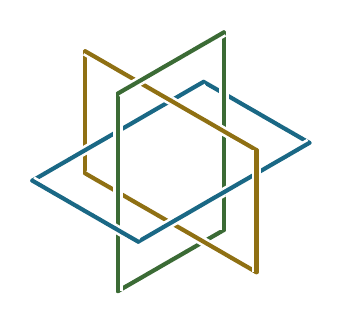
\begin{tikzpicture}
\draw[white,line width=3.4pt] (0.511,0.960)--(0.415,1.015);
\draw[ringB,line width=1.5pt,line cap=round] (0.511,0.960)--(0.415,1.015);
\draw[white,line width=3.4pt] (-1.087,-0.037)--(-1.087,-0.148);
\draw[ringC,line width=1.5pt,line cap=round] (-1.087,-0.037)--(-1.087,-0.148);
\draw[white,line width=3.4pt] (0.576,-0.923)--(0.672,-0.867);
\draw[ringD,line width=1.5pt,line cap=round] (0.576,-0.923)--(0.672,-0.867);
\draw[white,line width=3.4pt] (0.415,1.015)--(0.260,0.926);
\draw[ringB,line width=1.5pt,line cap=round] (0.415,1.015)--(0.260,0.926);
\draw[white,line width=3.4pt] (-1.087,-0.148)--(-0.932,-0.238);
\draw[ringC,line width=1.5pt,line cap=round] (-1.087,-0.148)--(-0.932,-0.238);
\draw[white,line width=3.4pt] (0.672,-0.867)--(0.672,-0.688);
\draw[ringD,line width=1.5pt,line cap=round] (0.672,-0.867)--(0.672,-0.688);
\draw[white,line width=3.4pt] (0.607,0.905)--(0.511,0.960);
\draw[ringB,line width=1.5pt,line cap=round] (0.607,0.905)--(0.511,0.960);
\draw[white,line width=3.4pt] (-1.087,0.073)--(-1.087,-0.037);
\draw[ringC,line width=1.5pt,line cap=round] (-1.087,0.073)--(-1.087,-0.037);
\draw[white,line width=3.4pt] (0.480,-0.978)--(0.576,-0.923);
\draw[ringD,line width=1.5pt,line cap=round] (0.480,-0.978)--(0.576,-0.923);
\draw[white,line width=3.4pt] (0.260,0.926)--(0.105,0.836);
\draw[ringB,line width=1.5pt,line cap=round] (0.260,0.926)--(0.105,0.836);
\draw[white,line width=3.4pt] (-0.932,-0.238)--(-0.776,-0.327);
\draw[ringC,line width=1.5pt,line cap=round] (-0.932,-0.238)--(-0.776,-0.327);
\draw[white,line width=3.4pt] (0.672,-0.688)--(0.672,-0.509);
\draw[ringD,line width=1.5pt,line cap=round] (0.672,-0.688)--(0.672,-0.509);
\draw[white,line width=3.4pt] (0.703,0.849)--(0.607,0.905);
\draw[ringB,line width=1.5pt,line cap=round] (0.703,0.849)--(0.607,0.905);
\draw[white,line width=3.4pt] (-1.087,0.184)--(-1.087,0.073);
\draw[ringC,line width=1.5pt,line cap=round] (-1.087,0.184)--(-1.087,0.073);
\draw[white,line width=3.4pt] (0.384,-1.033)--(0.480,-0.978);
\draw[ringD,line width=1.5pt,line cap=round] (0.384,-1.033)--(0.480,-0.978);
\draw[white,line width=3.4pt] (0.799,0.794)--(0.703,0.849);
\draw[ringB,line width=1.5pt,line cap=round] (0.799,0.794)--(0.703,0.849);
\draw[white,line width=3.4pt] (-1.087,0.295)--(-1.087,0.184);
\draw[ringC,line width=1.5pt,line cap=round] (-1.087,0.295)--(-1.087,0.184);
\draw[white,line width=3.4pt] (0.288,-1.089)--(0.384,-1.033);
\draw[ringD,line width=1.5pt,line cap=round] (0.288,-1.089)--(0.384,-1.033);
\draw[white,line width=3.4pt] (0.105,0.836)--(-0.051,0.746);
\draw[ringB,line width=1.5pt,line cap=round] (0.105,0.836)--(-0.051,0.746);
\draw[white,line width=3.4pt] (-0.776,-0.327)--(-0.621,-0.417);
\draw[ringC,line width=1.5pt,line cap=round] (-0.776,-0.327)--(-0.621,-0.417);
\draw[white,line width=3.4pt] (0.672,-0.509)--(0.672,-0.329);
\draw[ringD,line width=1.5pt,line cap=round] (0.672,-0.509)--(0.672,-0.329);
\draw[white,line width=3.4pt] (0.895,0.738)--(0.799,0.794);
\draw[ringB,line width=1.5pt,line cap=round] (0.895,0.738)--(0.799,0.794);
\draw[white,line width=3.4pt] (-1.087,0.406)--(-1.087,0.295);
\draw[ringC,line width=1.5pt,line cap=round] (-1.087,0.406)--(-1.087,0.295);
\draw[white,line width=3.4pt] (0.192,-1.144)--(0.288,-1.089);
\draw[ringD,line width=1.5pt,line cap=round] (0.192,-1.144)--(0.288,-1.089);
\draw[white,line width=3.4pt] (0.991,0.683)--(0.895,0.738);
\draw[ringB,line width=1.5pt,line cap=round] (0.991,0.683)--(0.895,0.738);
\draw[white,line width=3.4pt] (-1.087,0.517)--(-1.087,0.406);
\draw[ringC,line width=1.5pt,line cap=round] (-1.087,0.517)--(-1.087,0.406);
\draw[white,line width=3.4pt] (0.096,-1.200)--(0.192,-1.144);
\draw[ringD,line width=1.5pt,line cap=round] (0.096,-1.200)--(0.192,-1.144);
\draw[white,line width=3.4pt] (-0.051,0.746)--(-0.206,0.657);
\draw[ringB,line width=1.5pt,line cap=round] (-0.051,0.746)--(-0.206,0.657);
\draw[white,line width=3.4pt] (-0.621,-0.417)--(-0.466,-0.507);
\draw[ringC,line width=1.5pt,line cap=round] (-0.621,-0.417)--(-0.466,-0.507);
\draw[white,line width=3.4pt] (0.672,-0.329)--(0.672,-0.150);
\draw[ringD,line width=1.5pt,line cap=round] (0.672,-0.329)--(0.672,-0.150);
\draw[white,line width=3.4pt] (1.087,0.628)--(0.991,0.683);
\draw[ringB,line width=1.5pt,line cap=round] (1.087,0.628)--(0.991,0.683);
\draw[white,line width=3.4pt] (-1.087,0.628)--(-1.087,0.517);
\draw[ringC,line width=1.5pt,line cap=round] (-1.087,0.628)--(-1.087,0.517);
\draw[white,line width=3.4pt] (0.000,-1.255)--(0.096,-1.200);
\draw[ringD,line width=1.5pt,line cap=round] (0.000,-1.255)--(0.096,-1.200);
\draw[white,line width=3.4pt] (-0.206,0.657)--(-0.361,0.567);
\draw[ringB,line width=1.5pt,line cap=round] (-0.206,0.657)--(-0.361,0.567);
\draw[white,line width=3.4pt] (-0.466,-0.507)--(-0.311,-0.596);
\draw[ringC,line width=1.5pt,line cap=round] (-0.466,-0.507)--(-0.311,-0.596);
\draw[white,line width=3.4pt] (0.672,-0.150)--(0.672,0.029);
\draw[ringD,line width=1.5pt,line cap=round] (0.672,-0.150)--(0.672,0.029);
\draw[white,line width=3.4pt] (1.183,0.572)--(1.087,0.628);
\draw[ringB,line width=1.5pt,line cap=round] (1.183,0.572)--(1.087,0.628);
\draw[white,line width=3.4pt] (-1.087,0.738)--(-1.087,0.628);
\draw[ringC,line width=1.5pt,line cap=round] (-1.087,0.738)--(-1.087,0.628);
\draw[white,line width=3.4pt] (-0.096,-1.310)--(0.000,-1.255);
\draw[ringD,line width=1.5pt,line cap=round] (-0.096,-1.310)--(0.000,-1.255);
\draw[white,line width=3.4pt] (1.279,0.517)--(1.183,0.572);
\draw[ringB,line width=1.5pt,line cap=round] (1.279,0.517)--(1.183,0.572);
\draw[white,line width=3.4pt] (-1.087,0.849)--(-1.087,0.738);
\draw[ringC,line width=1.5pt,line cap=round] (-1.087,0.849)--(-1.087,0.738);
\draw[white,line width=3.4pt] (-0.192,-1.366)--(-0.096,-1.310);
\draw[ringD,line width=1.5pt,line cap=round] (-0.192,-1.366)--(-0.096,-1.310);
\draw[white,line width=3.4pt] (-0.361,0.567)--(-0.516,0.477);
\draw[ringB,line width=1.5pt,line cap=round] (-0.361,0.567)--(-0.516,0.477);
\draw[white,line width=3.4pt] (-0.311,-0.596)--(-0.155,-0.686);
\draw[ringC,line width=1.5pt,line cap=round] (-0.311,-0.596)--(-0.155,-0.686);
\draw[white,line width=3.4pt] (0.672,0.029)--(0.672,0.209);
\draw[ringD,line width=1.5pt,line cap=round] (0.672,0.029)--(0.672,0.209);
\draw[white,line width=3.4pt] (1.375,0.461)--(1.279,0.517);
\draw[ringB,line width=1.5pt,line cap=round] (1.375,0.461)--(1.279,0.517);
\draw[white,line width=3.4pt] (-1.087,0.960)--(-1.087,0.849);
\draw[ringC,line width=1.5pt,line cap=round] (-1.087,0.960)--(-1.087,0.849);
\draw[white,line width=3.4pt] (-0.288,-1.421)--(-0.192,-1.366);
\draw[ringD,line width=1.5pt,line cap=round] (-0.288,-1.421)--(-0.192,-1.366);
\draw[white,line width=3.4pt] (1.471,0.406)--(1.375,0.461);
\draw[ringB,line width=1.5pt,line cap=round] (1.471,0.406)--(1.375,0.461);
\draw[white,line width=3.4pt] (-1.087,1.071)--(-1.087,0.960);
\draw[ringC,line width=1.5pt,line cap=round] (-1.087,1.071)--(-1.087,0.960);
\draw[white,line width=3.4pt] (-0.384,-1.477)--(-0.288,-1.421);
\draw[ringD,line width=1.5pt,line cap=round] (-0.384,-1.477)--(-0.288,-1.421);
\draw[white,line width=3.4pt] (-0.516,0.477)--(-0.672,0.388);
\draw[ringB,line width=1.5pt,line cap=round] (-0.516,0.477)--(-0.672,0.388);
\draw[white,line width=3.4pt] (-0.155,-0.686)--(0.000,-0.776);
\draw[ringC,line width=1.5pt,line cap=round] (-0.155,-0.686)--(0.000,-0.776);
\draw[white,line width=3.4pt] (0.672,0.209)--(0.672,0.388);
\draw[ringD,line width=1.5pt,line cap=round] (0.672,0.209)--(0.672,0.388);
\draw[white,line width=3.4pt] (1.567,0.351)--(1.471,0.406);
\draw[ringB,line width=1.5pt,line cap=round] (1.567,0.351)--(1.471,0.406);
\draw[white,line width=3.4pt] (-1.087,1.182)--(-1.087,1.071);
\draw[ringC,line width=1.5pt,line cap=round] (-1.087,1.182)--(-1.087,1.071);
\draw[white,line width=3.4pt] (-0.480,-1.532)--(-0.384,-1.477);
\draw[ringD,line width=1.5pt,line cap=round] (-0.480,-1.532)--(-0.384,-1.477);
\draw[white,line width=3.4pt] (-0.672,0.388)--(-0.827,0.298);
\draw[ringB,line width=1.5pt,line cap=round] (-0.672,0.388)--(-0.827,0.298);
\draw[white,line width=3.4pt] (0.000,-0.776)--(0.155,-0.865);
\draw[ringC,line width=1.5pt,line cap=round] (0.000,-0.776)--(0.155,-0.865);
\draw[white,line width=3.4pt] (0.672,0.388)--(0.672,0.567);
\draw[ringD,line width=1.5pt,line cap=round] (0.672,0.388)--(0.672,0.567);
\draw[white,line width=3.4pt] (1.663,0.295)--(1.567,0.351);
\draw[ringB,line width=1.5pt,line cap=round] (1.663,0.295)--(1.567,0.351);
\draw[white,line width=3.4pt] (-1.087,1.292)--(-1.087,1.182);
\draw[ringC,line width=1.5pt,line cap=round] (-1.087,1.292)--(-1.087,1.182);
\draw[white,line width=3.4pt] (-0.576,-1.587)--(-0.480,-1.532);
\draw[ringD,line width=1.5pt,line cap=round] (-0.576,-1.587)--(-0.480,-1.532);
\draw[white,line width=3.4pt] (1.759,0.240)--(1.663,0.295);
\draw[ringB,line width=1.5pt,line cap=round] (1.759,0.240)--(1.663,0.295);
\draw[white,line width=3.4pt] (-1.087,1.403)--(-1.087,1.292);
\draw[ringC,line width=1.5pt,line cap=round] (-1.087,1.403)--(-1.087,1.292);
\draw[white,line width=3.4pt] (-0.672,-1.643)--(-0.576,-1.587);
\draw[ringD,line width=1.5pt,line cap=round] (-0.672,-1.643)--(-0.576,-1.587);
\draw[white,line width=3.4pt] (-0.827,0.298)--(-0.982,0.209);
\draw[ringB,line width=1.5pt,line cap=round] (-0.827,0.298)--(-0.982,0.209);
\draw[white,line width=3.4pt] (0.155,-0.865)--(0.311,-0.955);
\draw[ringC,line width=1.5pt,line cap=round] (0.155,-0.865)--(0.311,-0.955);
\draw[white,line width=3.4pt] (0.672,0.567)--(0.672,0.746);
\draw[ringD,line width=1.5pt,line cap=round] (0.672,0.567)--(0.672,0.746);
\draw[white,line width=3.4pt] (1.603,0.150)--(1.759,0.240);
\draw[ringB,line width=1.5pt,line cap=round] (1.603,0.150)--(1.759,0.240);
\draw[white,line width=3.4pt] (-0.932,1.314)--(-1.087,1.403);
\draw[ringC,line width=1.5pt,line cap=round] (-0.932,1.314)--(-1.087,1.403);
\draw[white,line width=3.4pt] (-0.672,-1.464)--(-0.672,-1.643);
\draw[ringD,line width=1.5pt,line cap=round] (-0.672,-1.464)--(-0.672,-1.643);
\draw[white,line width=3.4pt] (-0.982,0.209)--(-1.138,0.119);
\draw[ringB,line width=1.5pt,line cap=round] (-0.982,0.209)--(-1.138,0.119);
\draw[white,line width=3.4pt] (0.311,-0.955)--(0.466,-1.045);
\draw[ringC,line width=1.5pt,line cap=round] (0.311,-0.955)--(0.466,-1.045);
\draw[white,line width=3.4pt] (0.672,0.746)--(0.672,0.926);
\draw[ringD,line width=1.5pt,line cap=round] (0.672,0.746)--(0.672,0.926);
\draw[white,line width=3.4pt] (1.448,0.060)--(1.603,0.150);
\draw[ringB,line width=1.5pt,line cap=round] (1.448,0.060)--(1.603,0.150);
\draw[white,line width=3.4pt] (-0.776,1.224)--(-0.932,1.314);
\draw[ringC,line width=1.5pt,line cap=round] (-0.776,1.224)--(-0.932,1.314);
\draw[white,line width=3.4pt] (-0.672,-1.284)--(-0.672,-1.464);
\draw[ringD,line width=1.5pt,line cap=round] (-0.672,-1.284)--(-0.672,-1.464);
\draw[white,line width=3.4pt] (-1.138,0.119)--(-1.293,0.029);
\draw[ringB,line width=1.5pt,line cap=round] (-1.138,0.119)--(-1.293,0.029);
\draw[white,line width=3.4pt] (0.466,-1.045)--(0.621,-1.134);
\draw[ringC,line width=1.5pt,line cap=round] (0.466,-1.045)--(0.621,-1.134);
\draw[white,line width=3.4pt] (0.672,0.926)--(0.672,1.105);
\draw[ringD,line width=1.5pt,line cap=round] (0.672,0.926)--(0.672,1.105);
\draw[white,line width=3.4pt] (1.293,-0.029)--(1.448,0.060);
\draw[ringB,line width=1.5pt,line cap=round] (1.293,-0.029)--(1.448,0.060);
\draw[white,line width=3.4pt] (-0.621,1.134)--(-0.776,1.224);
\draw[ringC,line width=1.5pt,line cap=round] (-0.621,1.134)--(-0.776,1.224);
\draw[white,line width=3.4pt] (-0.672,-1.105)--(-0.672,-1.284);
\draw[ringD,line width=1.5pt,line cap=round] (-0.672,-1.105)--(-0.672,-1.284);
\draw[white,line width=3.4pt] (-1.293,0.029)--(-1.448,-0.060);
\draw[ringB,line width=1.5pt,line cap=round] (-1.293,0.029)--(-1.448,-0.060);
\draw[white,line width=3.4pt] (0.621,-1.134)--(0.776,-1.224);
\draw[ringC,line width=1.5pt,line cap=round] (0.621,-1.134)--(0.776,-1.224);
\draw[white,line width=3.4pt] (0.672,1.105)--(0.672,1.284);
\draw[ringD,line width=1.5pt,line cap=round] (0.672,1.105)--(0.672,1.284);
\draw[white,line width=3.4pt] (1.138,-0.119)--(1.293,-0.029);
\draw[ringB,line width=1.5pt,line cap=round] (1.138,-0.119)--(1.293,-0.029);
\draw[white,line width=3.4pt] (-0.466,1.045)--(-0.621,1.134);
\draw[ringC,line width=1.5pt,line cap=round] (-0.466,1.045)--(-0.621,1.134);
\draw[white,line width=3.4pt] (-0.672,-0.926)--(-0.672,-1.105);
\draw[ringD,line width=1.5pt,line cap=round] (-0.672,-0.926)--(-0.672,-1.105);
\draw[white,line width=3.4pt] (-1.448,-0.060)--(-1.603,-0.150);
\draw[ringB,line width=1.5pt,line cap=round] (-1.448,-0.060)--(-1.603,-0.150);
\draw[white,line width=3.4pt] (0.776,-1.224)--(0.932,-1.314);
\draw[ringC,line width=1.5pt,line cap=round] (0.776,-1.224)--(0.932,-1.314);
\draw[white,line width=3.4pt] (0.672,1.284)--(0.672,1.464);
\draw[ringD,line width=1.5pt,line cap=round] (0.672,1.284)--(0.672,1.464);
\draw[white,line width=3.4pt] (0.982,-0.209)--(1.138,-0.119);
\draw[ringB,line width=1.5pt,line cap=round] (0.982,-0.209)--(1.138,-0.119);
\draw[white,line width=3.4pt] (-0.311,0.955)--(-0.466,1.045);
\draw[ringC,line width=1.5pt,line cap=round] (-0.311,0.955)--(-0.466,1.045);
\draw[white,line width=3.4pt] (-0.672,-0.746)--(-0.672,-0.926);
\draw[ringD,line width=1.5pt,line cap=round] (-0.672,-0.746)--(-0.672,-0.926);
\draw[white,line width=3.4pt] (-1.603,-0.150)--(-1.759,-0.240);
\draw[ringB,line width=1.5pt,line cap=round] (-1.603,-0.150)--(-1.759,-0.240);
\draw[white,line width=3.4pt] (0.932,-1.314)--(1.087,-1.403);
\draw[ringC,line width=1.5pt,line cap=round] (0.932,-1.314)--(1.087,-1.403);
\draw[white,line width=3.4pt] (0.672,1.464)--(0.672,1.643);
\draw[ringD,line width=1.5pt,line cap=round] (0.672,1.464)--(0.672,1.643);
\draw[white,line width=3.4pt] (0.827,-0.298)--(0.982,-0.209);
\draw[ringB,line width=1.5pt,line cap=round] (0.827,-0.298)--(0.982,-0.209);
\draw[white,line width=3.4pt] (-0.155,0.865)--(-0.311,0.955);
\draw[ringC,line width=1.5pt,line cap=round] (-0.155,0.865)--(-0.311,0.955);
\draw[white,line width=3.4pt] (-0.672,-0.567)--(-0.672,-0.746);
\draw[ringD,line width=1.5pt,line cap=round] (-0.672,-0.567)--(-0.672,-0.746);
\draw[white,line width=3.4pt] (-1.759,-0.240)--(-1.663,-0.295);
\draw[ringB,line width=1.5pt,line cap=round] (-1.759,-0.240)--(-1.663,-0.295);
\draw[white,line width=3.4pt] (1.087,-1.403)--(1.087,-1.292);
\draw[ringC,line width=1.5pt,line cap=round] (1.087,-1.403)--(1.087,-1.292);
\draw[white,line width=3.4pt] (0.672,1.643)--(0.576,1.587);
\draw[ringD,line width=1.5pt,line cap=round] (0.672,1.643)--(0.576,1.587);
\draw[white,line width=3.4pt] (-1.663,-0.295)--(-1.567,-0.351);
\draw[ringB,line width=1.5pt,line cap=round] (-1.663,-0.295)--(-1.567,-0.351);
\draw[white,line width=3.4pt] (1.087,-1.292)--(1.087,-1.182);
\draw[ringC,line width=1.5pt,line cap=round] (1.087,-1.292)--(1.087,-1.182);
\draw[white,line width=3.4pt] (0.576,1.587)--(0.480,1.532);
\draw[ringD,line width=1.5pt,line cap=round] (0.576,1.587)--(0.480,1.532);
\draw[white,line width=3.4pt] (0.672,-0.388)--(0.827,-0.298);
\draw[ringB,line width=1.5pt,line cap=round] (0.672,-0.388)--(0.827,-0.298);
\draw[white,line width=3.4pt] (0.000,0.776)--(-0.155,0.865);
\draw[ringC,line width=1.5pt,line cap=round] (0.000,0.776)--(-0.155,0.865);
\draw[white,line width=3.4pt] (-0.672,-0.388)--(-0.672,-0.567);
\draw[ringD,line width=1.5pt,line cap=round] (-0.672,-0.388)--(-0.672,-0.567);
\draw[white,line width=3.4pt] (-1.567,-0.351)--(-1.471,-0.406);
\draw[ringB,line width=1.5pt,line cap=round] (-1.567,-0.351)--(-1.471,-0.406);
\draw[white,line width=3.4pt] (1.087,-1.182)--(1.087,-1.071);
\draw[ringC,line width=1.5pt,line cap=round] (1.087,-1.182)--(1.087,-1.071);
\draw[white,line width=3.4pt] (0.480,1.532)--(0.384,1.477);
\draw[ringD,line width=1.5pt,line cap=round] (0.480,1.532)--(0.384,1.477);
\draw[white,line width=3.4pt] (0.516,-0.477)--(0.672,-0.388);
\draw[ringB,line width=1.5pt,line cap=round] (0.516,-0.477)--(0.672,-0.388);
\draw[white,line width=3.4pt] (0.155,0.686)--(0.000,0.776);
\draw[ringC,line width=1.5pt,line cap=round] (0.155,0.686)--(0.000,0.776);
\draw[white,line width=3.4pt] (-0.672,-0.209)--(-0.672,-0.388);
\draw[ringD,line width=1.5pt,line cap=round] (-0.672,-0.209)--(-0.672,-0.388);
\draw[white,line width=3.4pt] (-1.471,-0.406)--(-1.375,-0.461);
\draw[ringB,line width=1.5pt,line cap=round] (-1.471,-0.406)--(-1.375,-0.461);
\draw[white,line width=3.4pt] (1.087,-1.071)--(1.087,-0.960);
\draw[ringC,line width=1.5pt,line cap=round] (1.087,-1.071)--(1.087,-0.960);
\draw[white,line width=3.4pt] (0.384,1.477)--(0.288,1.421);
\draw[ringD,line width=1.5pt,line cap=round] (0.384,1.477)--(0.288,1.421);
\draw[white,line width=3.4pt] (-1.375,-0.461)--(-1.279,-0.517);
\draw[ringB,line width=1.5pt,line cap=round] (-1.375,-0.461)--(-1.279,-0.517);
\draw[white,line width=3.4pt] (1.087,-0.960)--(1.087,-0.849);
\draw[ringC,line width=1.5pt,line cap=round] (1.087,-0.960)--(1.087,-0.849);
\draw[white,line width=3.4pt] (0.288,1.421)--(0.192,1.366);
\draw[ringD,line width=1.5pt,line cap=round] (0.288,1.421)--(0.192,1.366);
\draw[white,line width=3.4pt] (0.361,-0.567)--(0.516,-0.477);
\draw[ringB,line width=1.5pt,line cap=round] (0.361,-0.567)--(0.516,-0.477);
\draw[white,line width=3.4pt] (0.311,0.596)--(0.155,0.686);
\draw[ringC,line width=1.5pt,line cap=round] (0.311,0.596)--(0.155,0.686);
\draw[white,line width=3.4pt] (-0.672,-0.029)--(-0.672,-0.209);
\draw[ringD,line width=1.5pt,line cap=round] (-0.672,-0.029)--(-0.672,-0.209);
\draw[white,line width=3.4pt] (-1.279,-0.517)--(-1.183,-0.572);
\draw[ringB,line width=1.5pt,line cap=round] (-1.279,-0.517)--(-1.183,-0.572);
\draw[white,line width=3.4pt] (1.087,-0.849)--(1.087,-0.738);
\draw[ringC,line width=1.5pt,line cap=round] (1.087,-0.849)--(1.087,-0.738);
\draw[white,line width=3.4pt] (0.192,1.366)--(0.096,1.310);
\draw[ringD,line width=1.5pt,line cap=round] (0.192,1.366)--(0.096,1.310);
\draw[white,line width=3.4pt] (-1.183,-0.572)--(-1.087,-0.628);
\draw[ringB,line width=1.5pt,line cap=round] (-1.183,-0.572)--(-1.087,-0.628);
\draw[white,line width=3.4pt] (1.087,-0.738)--(1.087,-0.628);
\draw[ringC,line width=1.5pt,line cap=round] (1.087,-0.738)--(1.087,-0.628);
\draw[white,line width=3.4pt] (0.096,1.310)--(0.000,1.255);
\draw[ringD,line width=1.5pt,line cap=round] (0.096,1.310)--(0.000,1.255);
\draw[white,line width=3.4pt] (0.206,-0.657)--(0.361,-0.567);
\draw[ringB,line width=1.5pt,line cap=round] (0.206,-0.657)--(0.361,-0.567);
\draw[white,line width=3.4pt] (0.466,0.507)--(0.311,0.596);
\draw[ringC,line width=1.5pt,line cap=round] (0.466,0.507)--(0.311,0.596);
\draw[white,line width=3.4pt] (-0.672,0.150)--(-0.672,-0.029);
\draw[ringD,line width=1.5pt,line cap=round] (-0.672,0.150)--(-0.672,-0.029);
\draw[white,line width=3.4pt] (-1.087,-0.628)--(-0.991,-0.683);
\draw[ringB,line width=1.5pt,line cap=round] (-1.087,-0.628)--(-0.991,-0.683);
\draw[white,line width=3.4pt] (1.087,-0.628)--(1.087,-0.517);
\draw[ringC,line width=1.5pt,line cap=round] (1.087,-0.628)--(1.087,-0.517);
\draw[white,line width=3.4pt] (0.000,1.255)--(-0.096,1.200);
\draw[ringD,line width=1.5pt,line cap=round] (0.000,1.255)--(-0.096,1.200);
\draw[white,line width=3.4pt] (0.051,-0.746)--(0.206,-0.657);
\draw[ringB,line width=1.5pt,line cap=round] (0.051,-0.746)--(0.206,-0.657);
\draw[white,line width=3.4pt] (0.621,0.417)--(0.466,0.507);
\draw[ringC,line width=1.5pt,line cap=round] (0.621,0.417)--(0.466,0.507);
\draw[white,line width=3.4pt] (-0.672,0.329)--(-0.672,0.150);
\draw[ringD,line width=1.5pt,line cap=round] (-0.672,0.329)--(-0.672,0.150);
\draw[white,line width=3.4pt] (-0.991,-0.683)--(-0.895,-0.738);
\draw[ringB,line width=1.5pt,line cap=round] (-0.991,-0.683)--(-0.895,-0.738);
\draw[white,line width=3.4pt] (1.087,-0.517)--(1.087,-0.406);
\draw[ringC,line width=1.5pt,line cap=round] (1.087,-0.517)--(1.087,-0.406);
\draw[white,line width=3.4pt] (-0.096,1.200)--(-0.192,1.144);
\draw[ringD,line width=1.5pt,line cap=round] (-0.096,1.200)--(-0.192,1.144);
\draw[white,line width=3.4pt] (-0.895,-0.738)--(-0.799,-0.794);
\draw[ringB,line width=1.5pt,line cap=round] (-0.895,-0.738)--(-0.799,-0.794);
\draw[white,line width=3.4pt] (1.087,-0.406)--(1.087,-0.295);
\draw[ringC,line width=1.5pt,line cap=round] (1.087,-0.406)--(1.087,-0.295);
\draw[white,line width=3.4pt] (-0.192,1.144)--(-0.288,1.089);
\draw[ringD,line width=1.5pt,line cap=round] (-0.192,1.144)--(-0.288,1.089);
\draw[white,line width=3.4pt] (-0.105,-0.836)--(0.051,-0.746);
\draw[ringB,line width=1.5pt,line cap=round] (-0.105,-0.836)--(0.051,-0.746);
\draw[white,line width=3.4pt] (0.776,0.327)--(0.621,0.417);
\draw[ringC,line width=1.5pt,line cap=round] (0.776,0.327)--(0.621,0.417);
\draw[white,line width=3.4pt] (-0.672,0.509)--(-0.672,0.329);
\draw[ringD,line width=1.5pt,line cap=round] (-0.672,0.509)--(-0.672,0.329);
\draw[white,line width=3.4pt] (-0.799,-0.794)--(-0.703,-0.849);
\draw[ringB,line width=1.5pt,line cap=round] (-0.799,-0.794)--(-0.703,-0.849);
\draw[white,line width=3.4pt] (1.087,-0.295)--(1.087,-0.184);
\draw[ringC,line width=1.5pt,line cap=round] (1.087,-0.295)--(1.087,-0.184);
\draw[white,line width=3.4pt] (-0.288,1.089)--(-0.384,1.033);
\draw[ringD,line width=1.5pt,line cap=round] (-0.288,1.089)--(-0.384,1.033);
\draw[white,line width=3.4pt] (-0.703,-0.849)--(-0.607,-0.905);
\draw[ringB,line width=1.5pt,line cap=round] (-0.703,-0.849)--(-0.607,-0.905);
\draw[white,line width=3.4pt] (1.087,-0.184)--(1.087,-0.073);
\draw[ringC,line width=1.5pt,line cap=round] (1.087,-0.184)--(1.087,-0.073);
\draw[white,line width=3.4pt] (-0.384,1.033)--(-0.480,0.978);
\draw[ringD,line width=1.5pt,line cap=round] (-0.384,1.033)--(-0.480,0.978);
\draw[white,line width=3.4pt] (-0.260,-0.926)--(-0.105,-0.836);
\draw[ringB,line width=1.5pt,line cap=round] (-0.260,-0.926)--(-0.105,-0.836);
\draw[white,line width=3.4pt] (0.932,0.238)--(0.776,0.327);
\draw[ringC,line width=1.5pt,line cap=round] (0.932,0.238)--(0.776,0.327);
\draw[white,line width=3.4pt] (-0.672,0.688)--(-0.672,0.509);
\draw[ringD,line width=1.5pt,line cap=round] (-0.672,0.688)--(-0.672,0.509);
\draw[white,line width=3.4pt] (-0.607,-0.905)--(-0.511,-0.960);
\draw[ringB,line width=1.5pt,line cap=round] (-0.607,-0.905)--(-0.511,-0.960);
\draw[white,line width=3.4pt] (1.087,-0.073)--(1.087,0.037);
\draw[ringC,line width=1.5pt,line cap=round] (1.087,-0.073)--(1.087,0.037);
\draw[white,line width=3.4pt] (-0.480,0.978)--(-0.576,0.923);
\draw[ringD,line width=1.5pt,line cap=round] (-0.480,0.978)--(-0.576,0.923);
\draw[white,line width=3.4pt] (-0.415,-1.015)--(-0.260,-0.926);
\draw[ringB,line width=1.5pt,line cap=round] (-0.415,-1.015)--(-0.260,-0.926);
\draw[white,line width=3.4pt] (1.087,0.148)--(0.932,0.238);
\draw[ringC,line width=1.5pt,line cap=round] (1.087,0.148)--(0.932,0.238);
\draw[white,line width=3.4pt] (-0.672,0.867)--(-0.672,0.688);
\draw[ringD,line width=1.5pt,line cap=round] (-0.672,0.867)--(-0.672,0.688);
\draw[white,line width=3.4pt] (-0.511,-0.960)--(-0.415,-1.015);
\draw[ringB,line width=1.5pt,line cap=round] (-0.511,-0.960)--(-0.415,-1.015);
\draw[white,line width=3.4pt] (1.087,0.037)--(1.087,0.148);
\draw[ringC,line width=1.5pt,line cap=round] (1.087,0.037)--(1.087,0.148);
\draw[white,line width=3.4pt] (-0.576,0.923)--(-0.672,0.867);
\draw[ringD,line width=1.5pt,line cap=round] (-0.576,0.923)--(-0.672,0.867);
\end{tikzpicture}

\caption{The standard diagram of the Borromean rings $\Bor$. Each component
passes over one neighbour and under the other, cyclically. No two of the three
are linked, yet all three together cannot be separated. Here and throughout,
over and under are shown only by the break in the lower strand; the colours
distinguish components and carry no other information.}
\label{fig:borromean}
\end{figure}

The \emph{linking number} $\lk(K_i,K_j)\in\ZZ$ of two oriented components is
half the sum of the signs of the crossings between them in any diagram; it is an
invariant of the link, and it vanishes for every pair of $\Bor$. Where a finer
measure is needed we use Milnor's triple invariant. If all the pairwise linking
numbers of a link vanish, then for distinct $i,j,k$ the invariant
$\bar\mu(ijk)\in\ZZ$ of~\cite{milnor1954,milnor1957} is defined with no
indeterminacy, it is unchanged by an orientation-preserving diffeomorphism of
$\RR^3$, and it is alternating: interchanging two of its three indices reverses
its sign. For the Borromean rings $\bar\mu(123)=\pm1$, the sign depending on the
chosen orientations and diagram.

Finally, let $\Tet\le SO(3)$ denote the rotation group of a regular tetrahedron:
the identity, eight rotations through $\pm120^\circ$ about the four axes joining
a vertex to the centre of the opposite face, and three rotations through
$180^\circ$ about the axes joining midpoints of opposite edges, so
$\abs{\Tet}=12$ and $\Tet\cong A_4$. An embedded link $L\subset\RR^3$ is
\emph{$\Tet$-symmetric} if $g(L)=L$ as a set for every $g\in\Tet$; this induces
a homomorphism $\rho\colon\Tet\to S_n$ by $g(K_i)=K_{\rho(g)(i)}$. Note that
symmetry is a property of an embedding and not of an equivalence class: a link
type ``has tetrahedral symmetry'' when some representative embedding does.

\section{The problem, and two things one need not assume}\label{sec:problem}

\begin{lemma}\label{lem:pairs}
If every three-component sublink of $L$ is $\Bor$, then $\lk(K_i,K_j)=0$ for
every pair, and indeed every two-component sublink of $L$ is the unlink $U_2$.
\end{lemma}

\begin{proof}
Any two-element subset of $\{1,2,3,4\}$ is contained in a three-element subset
$S$. By hypothesis $L_S\cong\Bor$, and every two-component sublink of $\Bor$ is
$U_2$. Sublinks of equivalent links are equivalent, so the two-component
sublinks of $L$ are each $U_2$.
\end{proof}

\begin{lemma}\label{lem:transitive}
Let $L$ have four components and let $\rho\colon\Tet\to S_4$ be injective. Then
$\rho(\Tet)=A_4$, the action on components is transitive, and the stabiliser of
each component is cyclic of order $3$, generated by a rotation through
$120^\circ$ about one of the four vertex-to-face axes.
\end{lemma}

\begin{proof}
$\rho(\Tet)$ is a subgroup of $S_4$ isomorphic to $A_4$, hence of order $12$ and
of index $2$; the only such subgroup of $S_4$ is $A_4$ itself. The action of
$A_4$ on four points is transitive, so by orbit--stabiliser each stabiliser has
order $3$. The elements of order $3$ in $\Tet$ are precisely the rotations
through $\pm120^\circ$ about the four vertex-to-face axes.
\end{proof}

So Problem~\ref{prob:main} needs only the two conditions stated. In particular
``pairwise unlinked'' is not an independent requirement, and transitivity on
components is a consequence rather than a hypothesis.

\section{The tetrahedral frame}\label{sec:frame}

Fix the regular tetrahedron $\Delta$ with vertices
\[
  v_1=(1,1,1),\quad v_2=(1,-1,-1),\quad v_3=(-1,1,-1),\quad v_4=(-1,-1,1),
\]
and let $F_i$ denote the face of $\Delta$ opposite $v_i$. By
Lemma~\ref{lem:transitive} we may label the components so that the stabiliser of
$K_i$ is generated by the rotation $r_i$ through $120^\circ$ about the axis
through $v_i$; we then say $K_i$ \emph{belongs to} $F_i$. In these coordinates
$r_1$ is the cyclic permutation of coordinates
\begin{equation}\label{eq:r1}
  r_1(x,y,z)=(z,x,y),
\end{equation}
and the three half-turns about the coordinate axes,
\begin{equation}\label{eq:halfturns}
  u_2(x,y,z)=(x,-y,-z),\qquad u_3(x,y,z)=(-x,y,-z),\qquad u_4(x,y,z)=(-x,-y,z),
\end{equation}
satisfy $u_i(v_1)=v_i$ and so represent the three nontrivial cosets of
$\langle r_1\rangle$ in $\Tet$.

\begin{lemma}[Generation principle]\label{lem:generate}
Let $K\subset\RR^3$ be any closed curve with $r_1(K)=K$, and set $K_1=K$,
$K_i=u_i(K)$ for $i=2,3,4$. If these four curves are pairwise disjoint, then
$L=K_1\sqcup K_2\sqcup K_3\sqcup K_4$ is $\Tet$-symmetric with $\rho$ injective.
\end{lemma}

\begin{proof}
Write $u_1=\mathrm{id}$. For $g\in\Tet$ and $i\in\{1,2,3,4\}$ there are a unique
$j$ and a unique $m\in\{0,1,2\}$ with $g\,u_i=u_j r_1^{\,m}$, because the $u_i$
represent the cosets of $\langle r_1\rangle$. Hence
$g(K_i)=g\,u_i(K)=u_j r_1^{\,m}(K)=u_j(K)=K_j$, so $g$ permutes the components.
The resulting permutation determines $g$ on cosets, and since $\Tet$ acts
faithfully on $\Tet/\langle r_1\rangle$, $\rho$ is injective.
\end{proof}

Lemma~\ref{lem:generate} is what makes the symmetry exact rather than
approximate: one designs a single $r_1$-invariant curve and the group produces
the rest, so there is no step at which the symmetry could be lost.

\begin{lemma}[Vertices and triples]\label{lem:vertices}
The map $S\mapsto v_k$, where $\{k\}=\{1,2,3,4\}\setminus S$, is a bijection
from three-element subsets of $\{1,2,3,4\}$ to vertices of $\Delta$, and it is
equivariant for the actions of $\Tet$. The components belonging to the three
faces meeting at $v_k$ are exactly $\{K_i : i\neq k\}$.
\end{lemma}

\begin{proof}
The three faces through $v_k$ are those containing $v_k$, namely $F_i$ for
$i\neq k$, since $F_k$ is the face opposite $v_k$. Complementation is a
bijection and commutes with the induced action.
\end{proof}

\begin{figure}[htbp]
\centering
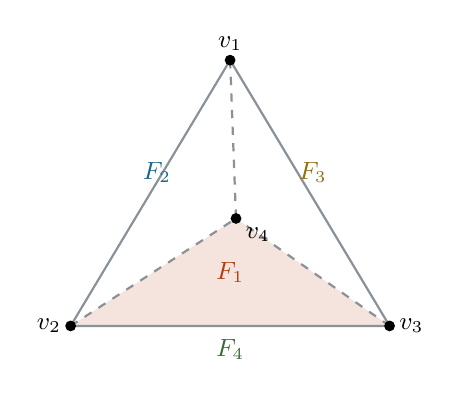
\begin{tikzpicture}[scale=1.5,line join=round]
  \coordinate (v1) at (0,1.5);
  \coordinate (v2) at (-1.35,-0.75);
  \coordinate (v3) at (1.35,-0.75);
  \coordinate (v4) at (0.05,0.16);
  \fill[ringA!14] (v2)--(v3)--(v4)--cycle;
  \draw[rulegrey,line width=0.8pt] (v1)--(v2)--(v3)--cycle;
  \draw[rulegrey,line width=0.8pt,dashed] (v1)--(v4) (v2)--(v4) (v3)--(v4);
  \foreach \p/\n/\pos in {v1/$v_1$/above, v2/$v_2$/left, v3/$v_3$/right, v4/$v_4$/{below right}}
    {\fill (\p) circle (1.3pt); \node[\pos,font=\small] at (\p) {\n};}
  \node[ringA,font=\small\bfseries] at (0.0,-0.30) {$F_1$};
  \node[ringB,font=\small] at (-0.62,0.55) {$F_2$};
  \node[ringC,font=\small] at (0.70,0.55) {$F_3$};
  \node[ringD,font=\small] at (0.0,-0.95) {$F_4$};
\end{tikzpicture}
\hspace{1.1cm}
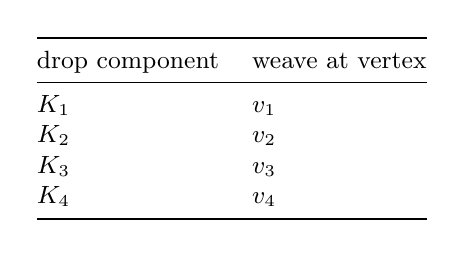
\begin{tikzpicture}[scale=0.92]
  \node[font=\small,align=left] at (0,0)
  {\begin{tabular}{@{}ll@{}}
    \toprule
    drop component & weave at vertex\\
    \midrule
    $K_1$ & $v_1$\\
    $K_2$ & $v_2$\\
    $K_3$ & $v_3$\\
    $K_4$ & $v_4$\\
    \bottomrule
  \end{tabular}};
\end{tikzpicture}
\caption{One component per face. Component $K_i$ belongs to the face $F_i$
opposite the vertex $v_i$. Deleting $K_k$ leaves the three components belonging
to the three faces that meet at $v_k$, so the four instances of condition~(i)
correspond to the four vertices, and the symmetry group permutes them
transitively.}
\label{fig:tetra}
\end{figure}

\section{The symmetry is compatible with the required linking}\label{sec:milnor}

Before constructing anything it is worth checking that conditions~(i) and~(ii)
are not in conflict, since a symmetry constrains the invariants of a link and
could in principle force them to vanish. They are not in conflict, and the
reason the check is clean is the following.

\begin{lemma}\label{lem:orient}
The components of a $\Tet$-symmetric four-component link may be oriented so
that every $g\in\Tet$ preserves the orientation of every component it maps to
itself, and carries chosen orientations to chosen orientations throughout.
\end{lemma}

\begin{proof}
An equivariant choice of orientations is a section of the associated
$\{\pm1\}$-bundle over the component set $\Tet/\langle r_1\rangle$, and such
bundles are classified by $\mathrm{Hom}(\langle r_1\rangle,\{\pm1\})$. Since
$\langle r_1\rangle$ has order $3$, which is odd, that group is trivial, so the
bundle is trivial and a section exists.
\end{proof}

With orientations so chosen, every $g\in\Tet$ is an orientation-preserving
diffeomorphism of $\RR^3$ carrying oriented components to oriented components,
so for $\sigma=\rho(g)$,
\begin{equation}\label{eq:muequivariance}
  \bar\mu(\sigma i,\sigma j,\sigma k)=\bar\mu(i,j,k).
\end{equation}

\begin{proposition}\label{prop:milnor}
Let $L$ satisfy~(ii), with all pairwise linking numbers zero. Then the vector
\[
  \big(\bar\mu(234),\,\bar\mu(134),\,\bar\mu(124),\,\bar\mu(123)\big)
\]
lies in a one-dimensional subspace of $\RR^4$, spanned by $(-1,1,-1,1)$. In
particular condition~(i), which forces $\abs{\bar\mu(ijk)}=1$ on all four
triples, is compatible with~(ii), and it determines the four signs up to a
single global sign.
\end{proposition}

\begin{proof}
Since $\bar\mu$ is alternating it is determined by its values on the four
three-element subsets written in increasing order, which are the four
coordinates above. Equation~\eqref{eq:muequivariance} for $\sigma$ ranging over
$\rho(\Tet)=A_4$ is a system of linear equations in those four unknowns. Take
$\sigma=(123)$. Applying~\eqref{eq:muequivariance} to the triples $(1,2,4)$,
$(2,3,4)$ and $(3,1,4)$ in turn, and using that $\bar\mu$ is alternating to
re-sort indices, gives $\bar\mu(234)=\bar\mu(124)$ and
$\bar\mu(134)=-\bar\mu(124)$. Taking $\sigma=(234)$ and arguing the same way
gives $\bar\mu(123)=-\bar\mu(124)$. Since $(123)$ and $(234)$ generate $A_4$,
these are all the relations, and the solution space is spanned by
$(1,-1,1,-1)$ in the ordering above, equivalently by $(-1,1,-1,1)$.
\end{proof}

\section{Two obstructions}\label{sec:obstructions}

Both obstructions in this section say that an obvious economy is unavailable.
They are what force the construction of Section~\ref{sec:construction} to look
as elaborate as it does.

\subsection{The components cannot be flat and convex}

Call a closed curve \emph{convex planar} if it lies in a plane and bounds a
convex region there; equivalently, no straight line meets it in more than two
points. Triangles and ellipses are convex planar; a star-shaped polygon is not.

\begin{theorem}\label{thm:convex}
No $\Tet$-symmetric four-component link all of whose components are convex
planar satisfies condition~(i).
\end{theorem}

\begin{proof}
Let $a_i$ be the axis through $v_i$, so that $K_i$ is invariant under the
rotation $r_i$ of order $3$ about $a_i$.

\emph{Step 1: the planes are forced.} A planar simple closed curve spans a
unique plane $P_i$, and $r_i(K_i)=K_i$ forces $r_i(P_i)=P_i$. A rotation through
$120^\circ$ about $a_i$ carries a plane containing $a_i$ to a different such
plane, since $120^\circ\not\equiv0\pmod{180^\circ}$; hence $P_i\perp a_i$.

\emph{Step 2: the half-turn reverses the line of intersection.} For $i\neq j$
the axes $a_i,a_j$ meet at an angle $\arccos(-1/3)$, so $P_i$ and $P_j$ are not
parallel and $\ell=P_i\cap P_j$ is a line. There is a unique element $u\in\Tet$
of order $2$ with $u(K_i)=K_j$ and $u(K_j)=K_i$, namely the half-turn realising
the double transposition $(ij)(kl)$; let $b$ be its axis. Then $u(\ell)=\ell$. A
half-turn carries a line to itself only if the line is $b$, or meets $b$
orthogonally. The first is impossible, as $b$ lies in neither $P_i$ nor $P_j$;
in the second case $u|_\ell$ is the point reflection of $\ell$ in the point
$\ell\cap b$. Concretely, for $i=1$, $j=2$ we have $b$ the $x$-axis, and with
$P_1=\{x+y+z=c\}$ and $P_2=\{x-y-z=c\}$ one computes
$\ell=\{(c,s,-s):s\in\RR\}$, whose direction $(0,1,-1)$ is orthogonal to $b$ and
which meets $b$ at $(c,0,0)$.

\emph{Step 3: chords cannot nest.} Being convex, $K_i$ meets $\ell$ in at most
two points, so (generically) $K_i\cap\ell$ is the pair of endpoints of an
interval $I_i\subset\ell$, and likewise for $K_j$. Two disjoint convex planar
curves lying in distinct planes are linked precisely when $I_i$ and $I_j$
interleave, and unlinked precisely when the intervals nest or are disjoint. By
Step 2, $I_j$ is the image of $I_i$ under the point reflection in
$m=\ell\cap b$. Taking $m$ as the origin of a coordinate on $\ell$ and writing
$I_i=[\alpha,\beta]$, we get $I_j=[-\beta,-\alpha]$. For $I_i\subseteq I_j$ we
would need $-\beta\le\alpha$ and $\beta\le-\alpha$, that is
$\alpha+\beta\ge0$ and $\alpha+\beta\le0$; so $\alpha+\beta=0$, $I_i=I_j$, and
the two curves meet. Nesting is therefore unavailable
(Figure~\ref{fig:intervals}).

\emph{Step 4: neither survivor works.} The group $A_4$ is $2$-transitive on four
points, hence transitive on the six unordered pairs, so every pair falls into
the same one of the remaining two cases. If all pairs interleave then
$\lk(K_i,K_j)=\pm1$ for every pair, contradicting Lemma~\ref{lem:pairs}. If all
pairs are disjoint, then the convex disc $D_i\subset P_i$ bounded by $K_i$ meets
$P_j$ only in the filled interval $I_i$, which is disjoint from $K_j$; so $D_i$
is a disc bounded by $K_i$ and disjoint from every other component, every
three-component sublink is split, and no such sublink is $\Bor$.
\end{proof}

\begin{figure}[htbp]
\centering
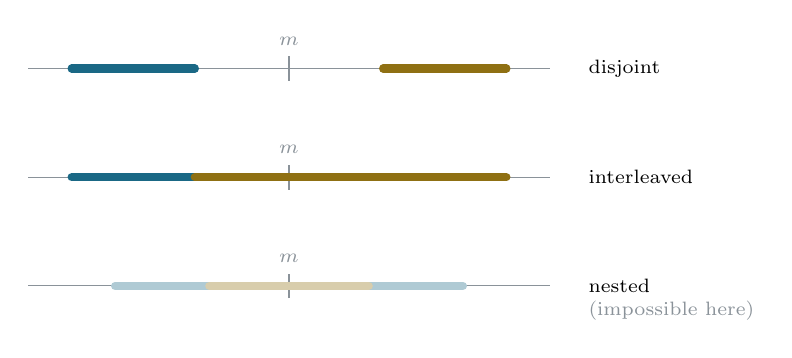
\begin{tikzpicture}[scale=0.92,font=\small]
  \foreach \y/\lab in {0/{disjoint}, -1.5/{interleaved}, -3.0/{nested}}
    {\draw[rulegrey] (-3.6,\y) -- (3.6,\y);
     \draw[rulegrey,line width=1pt] (0,\y-0.17) -- (0,\y+0.17);
     \node[rulegrey,font=\scriptsize] at (0,\y+0.38) {$m$};
     \node[anchor=west,font=\scriptsize] at (4.0,\y) {\lab};}
  % disjoint
  \draw[ringB,line width=3pt,line cap=round] (-3.0,0)--(-1.3,0);
  \draw[ringC,line width=3pt,line cap=round] (1.3,0)--(3.0,0);
  % interleaved
  \draw[ringB,line width=3pt,line cap=round] (-3.0,-1.5)--(1.3,-1.5);
  \draw[ringC,line width=3pt,line cap=round] (-1.3,-1.5)--(3.0,-1.5);
  % nested -- greyed, because it is the case the symmetry forbids
  \draw[ringB!35,line width=3pt,line cap=round] (-2.4,-3.0)--(2.4,-3.0);
  \draw[ringC!35,line width=3pt,line cap=round] (-1.1,-3.0)--(1.1,-3.0);
  \node[font=\scriptsize,anchor=west] at (4.0,-3.34) {\textcolor{rulegrey}{(impossible here)}};
\end{tikzpicture}
\caption{The three ways two intervals can sit on the line $\ell=P_i\cap P_j$.
The half-turn exchanging the two components reflects $\ell$ in the point $m$,
so one interval is the mirror image of the other through $m$. Disjoint and
interleaved configurations are compatible with that; nesting is not, and nesting
is the only one of the three that yields a Borromean triple.}
\label{fig:intervals}
\end{figure}

\subsection{The components cannot cross the minimum number of times}

Theorem~\ref{thm:convex} forces the components off their planes. The next
result forces them to cross each other more often than one might hope.

Suppose, as the picture in Figure~\ref{fig:tetra} suggests, that each component
runs along the boundary of its face. Two faces $F_i,F_j$ share an edge whose
endpoints are the two vertices $v_k,v_l$ with $\{k,l\}=\{1,2,3,4\}\setminus\{i,j\}$,
so the components $K_i$ and $K_j$ come close together near $v_k$ and near $v_l$
and nowhere else. The most economical diagram consistent with that picture is
one in which the three components at each vertex cross each other once apiece,
giving $4\times3=12$ crossings in all and exactly two crossings per pair --- the
fewest any link satisfying our conditions could have, since a pair crossing
fewer than twice has nonzero linking number or does not interact at all.

\begin{theorem}\label{thm:minimal}
There is no $\Tet$-symmetric diagram of a four-component link in which, for each
vertex $v_k$, the three components $\{K_i:i\neq k\}$ pairwise cross exactly once
near $v_k$, and no crossings occur elsewhere.
\end{theorem}

\begin{proof}
Fix such a diagram. Near $v_k$ the three components cross pairwise once, so the
relation ``$K_i$ passes over $K_j$ near $v_k$'' is a tournament on three
elements. The stabiliser of $v_k$ in $\Tet$ is $\langle r_k\rangle$, which
permutes those three components in a $3$-cycle and preserves the relation; a
$3$-cycle preserves no linear order on three elements, so the relation is a
cyclic order, and there are exactly two of them. Since $\Tet$ is transitive on
the vertices of $\Delta$, the choice at one vertex determines the choice at all
four, so there are exactly two diagrams to consider, interchanged by reversing
every cyclic order.

Each pair $\{K_i,K_j\}$ crosses exactly twice, at $v_k$ and at $v_l$. Two
crossings between distinct components contribute $\pm1$ each to
$2\lk(K_i,K_j)$, and the two contributions cancel exactly when the \emph{same}
component passes over at both crossings. By Lemma~\ref{lem:pairs} we therefore
need the over-strand of the pair $\{K_i,K_j\}$ to be the same at $v_k$ and at
$v_l$.

Take the cyclic order at $v_k$ to be the orbit of $r_k$, the rotation through
$+120^\circ$ about the axis through $v_k$. In the coordinates
of~\eqref{eq:r1}--\eqref{eq:halfturns} these rotations act on indices as
\[
  r_1=(2\,3\,4),\qquad r_2=(1\,4\,3),\qquad r_3=(1\,2\,4),\qquad r_4=(1\,3\,2),
\]
and the over-strand of a pair at a vertex is read off from the corresponding
cyclic order. The six pairs give
\begin{center}\small
\begin{tabular}{@{}lccc@{}}
\toprule
pair & vertices & over at the first & over at the second\\
\midrule
$\{K_1,K_2\}$ & $v_3,v_4$ & $K_1$ & $K_2$\\
$\{K_1,K_3\}$ & $v_2,v_4$ & $K_3$ & $K_1$\\
$\{K_1,K_4\}$ & $v_2,v_3$ & $K_1$ & $K_4$\\
$\{K_2,K_3\}$ & $v_1,v_4$ & $K_2$ & $K_3$\\
$\{K_2,K_4\}$ & $v_1,v_3$ & $K_4$ & $K_2$\\
$\{K_3,K_4\}$ & $v_1,v_2$ & $K_3$ & $K_4$\\
\bottomrule
\end{tabular}
\end{center}
In every row the over-strand changes, so every pair has linking number $\pm1$.
Reversing all four cyclic orders exchanges the two columns and changes nothing.
Both diagrams are therefore excluded by Lemma~\ref{lem:pairs}.
\end{proof}

Theorems~\ref{thm:convex} and~\ref{thm:minimal} together explain the shape of
what follows: the components must leave their planes, and they must meet each
other more than twice per pair.

\section{The link}\label{sec:construction}

\begin{theorem}\label{thm:main}
Let
\[
  p=(3,-1,-1),\qquad q=(-1,0,-2),
\]
let $K_1$ be the closed hexagon through
\[
  p,\quad q,\quad r_1(p),\quad r_1(q),\quad r_1^2(p),\quad r_1^2(q)
\]
in that cyclic order, and let $K_i=u_i(K_1)$ for $i=2,3,4$ as
in~\eqref{eq:halfturns}. Then $L=K_1\sqcup K_2\sqcup K_3\sqcup K_4$ is a
four-component link with all twenty-four vertices in $\ZZ^3$, it is
$\Tet$-symmetric with $\rho$ injective, all six of its pairwise linking numbers
vanish, and each of its four three-component sublinks is the Borromean rings.
\end{theorem}

Written out, with $r_1(x,y,z)=(z,x,y)$, the four hexagons are the rows of
Table~\ref{tab:coords}; Figure~\ref{fig:link} shows the link along two of its
symmetry axes.

\begin{table}[htbp]
\centering\small
\begin{tabular}{@{}ll@{}}
\toprule
component & vertices\\
\midrule
\textcolor{ringA}{$K_1$} & $(3,-1,-1)$\quad $(-1,0,-2)$\quad $(-1,3,-1)$\quad $(-2,-1,0)$\quad $(-1,-1,3)$\quad $(0,-2,-1)$\\
\textcolor{ringB}{$K_2$} & $(3,1,1)$\quad $(-1,0,2)$\quad $(-1,-3,1)$\quad $(-2,1,0)$\quad $(-1,1,-3)$\quad $(0,2,1)$\\
\textcolor{ringC}{$K_3$} & $(-3,-1,1)$\quad $(1,0,2)$\quad $(1,3,1)$\quad $(2,-1,0)$\quad $(1,-1,-3)$\quad $(0,-2,1)$\\
\textcolor{ringD}{$K_4$} & $(-3,1,-1)$\quad $(1,0,-2)$\quad $(1,-3,-1)$\quad $(2,1,0)$\quad $(1,1,3)$\quad $(0,2,-1)$\\
\bottomrule
\end{tabular}
\caption{The twenty-four vertices of $L$. Each row is a closed hexagon, listed
in cyclic order; $K_2,K_3,K_4$ are the images of $K_1$ under the half-turns
$u_2,u_3,u_4$ about the three coordinate axes.}
\label{tab:coords}
\end{table}

\begin{figure}[htbp]
\centering
\resizebox{0.70\linewidth}{!}{% generated by make-diagram.mjs -- do not edit
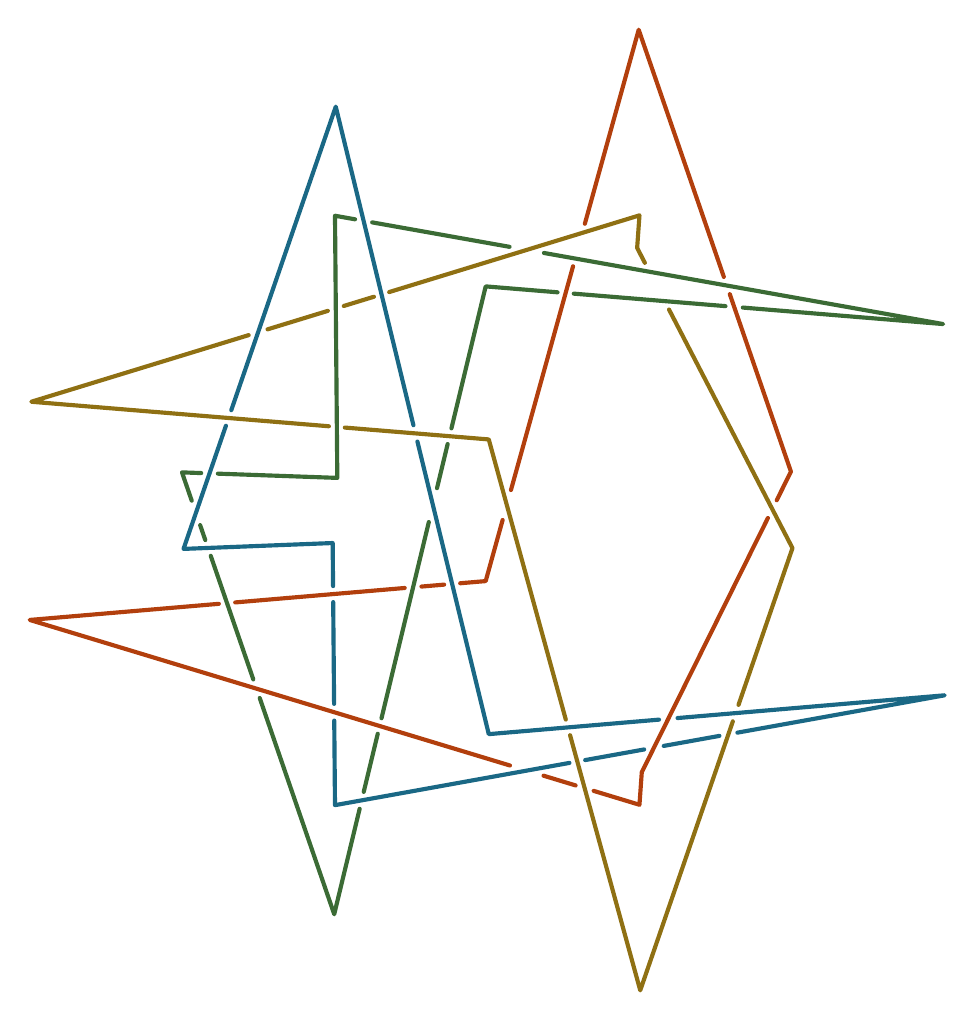
\begin{tikzpicture}
\draw[ringA,line width=1.5pt,line cap=round,line join=round] (1.0900,3.0988)--(0.3014,0.2570);
\draw[ringA,line width=1.5pt,line cap=round,line join=round] (0.1957,-0.1236)--(-0.0196,-0.8995)--(-0.3433,-0.9271);
\draw[ringA,line width=1.5pt,line cap=round,line join=round] (-0.5477,-0.9445)--(-0.8350,-0.9690);
\draw[ringA,line width=1.5pt,line cap=round,line join=round] (-1.0479,-0.9871)--(-3.2004,-1.1705);
\draw[ringA,line width=1.5pt,line cap=round,line join=round] (-3.4087,-1.1882)--(-5.8100,-1.3928)--(0.2890,-3.2417);
\draw[ringA,line width=1.5pt,line cap=round,line join=round] (0.7151,-3.3709)--(1.1224,-3.4944);
\draw[ringA,line width=1.5pt,line cap=round,line join=round] (1.3518,-3.5639)--(1.9334,-3.7403)--(1.9628,-3.3267)--(3.5646,-0.0985);
\draw[ringA,line width=1.5pt,line cap=round,line join=round] (3.6763,0.1267)--(3.8570,0.4908)--(3.0806,2.7443);
\draw[ringA,line width=1.5pt,line cap=round,line join=round] (3.0050,2.9637)--(1.9236,6.1025)--(1.2398,3.6386);
\draw[ringB,line width=1.5pt,line cap=round,line join=round] (-0.8865,0.8724)--(0.0196,-2.8432)--(2.1809,-2.6591);
\draw[ringB,line width=1.5pt,line cap=round,line join=round] (2.4172,-2.6389)--(5.8100,-2.3499)--(3.1771,-2.8243);
\draw[ringB,line width=1.5pt,line cap=round,line join=round] (2.9486,-2.8655)--(2.2416,-2.9929);
\draw[ringB,line width=1.5pt,line cap=round,line join=round] (1.9930,-3.0377)--(1.2442,-3.1726);
\draw[ringB,line width=1.5pt,line cap=round,line join=round] (1.0439,-3.2087)--(-1.9334,-3.7452)--(-1.9429,-2.6711);
\draw[ringB,line width=1.5pt,line cap=round,line join=round] (-1.9448,-2.4587)--(-1.9562,-1.1662);
\draw[ringB,line width=1.5pt,line cap=round,line join=round] (-1.9580,-0.9629)--(-1.9628,-0.4161)--(-3.8570,-0.4908)--(-3.3187,1.0728);
\draw[ringB,line width=1.5pt,line cap=round,line join=round] (-3.2507,1.2706)--(-1.9236,5.1257)--(-0.9371,1.0800);
\draw[ringC,line width=1.5pt,line cap=round,line join=round] (0.9977,-2.6581)--(0.0196,0.8995)--(-1.8083,1.0501);
\draw[ringC,line width=1.5pt,line cap=round,line join=round] (-2.0112,1.0668)--(-5.7904,1.3781)--(-3.0296,2.2242);
\draw[ringC,line width=1.5pt,line cap=round,line join=round] (-2.7899,2.2976)--(-2.0241,2.5323);
\draw[ringC,line width=1.5pt,line cap=round,line join=round] (-1.8219,2.5943)--(-1.4392,2.7116);
\draw[ringC,line width=1.5pt,line cap=round,line join=round] (-1.2451,2.7711)--(1.9334,3.7452)--(1.9040,3.3316)--(2.0019,3.1423);
\draw[ringC,line width=1.5pt,line cap=round,line join=round] (2.3085,2.5497)--(3.8766,-0.4810)--(3.1915,-2.4712);
\draw[ringC,line width=1.5pt,line cap=round,line join=round] (3.1193,-2.6809)--(1.9432,-6.0975)--(1.0523,-2.8570);
\draw[ringD,line width=1.5pt,line cap=round,line join=round] (-1.5683,-3.5764)--(-1.3903,-2.8386);
\draw[ringD,line width=1.5pt,line cap=round,line join=round] (-1.3426,-2.6412)--(-0.7416,-0.1496);
\draw[ringD,line width=1.5pt,line cap=round,line join=round] (-0.6378,0.2806)--(-0.5026,0.8408);
\draw[ringD,line width=1.5pt,line cap=round,line join=round] (-0.4545,1.0403)--(-0.0196,2.8432)--(0.8930,2.7680);
\draw[ringD,line width=1.5pt,line cap=round,line join=round] (1.0987,2.7511)--(3.0257,2.5924);
\draw[ringD,line width=1.5pt,line cap=round,line join=round] (3.2464,2.5742)--(5.7904,2.3647)--(0.7208,3.2675);
\draw[ringD,line width=1.5pt,line cap=round,line join=round] (0.2833,3.3455)--(-1.4609,3.6561);
\draw[ringD,line width=1.5pt,line cap=round,line join=round] (-1.6790,3.6950)--(-1.9334,3.7403)--(-1.9040,0.4111)--(-3.4208,0.4649);
\draw[ringD,line width=1.5pt,line cap=round,line join=round] (-3.6326,0.4724)--(-3.8766,0.4810)--(-3.7531,0.1225);
\draw[ringD,line width=1.5pt,line cap=round,line join=round] (-3.6458,-0.1888)--(-3.5805,-0.3785);
\draw[ringD,line width=1.5pt,line cap=round,line join=round] (-3.5115,-0.5786)--(-2.9710,-2.1476);
\draw[ringD,line width=1.5pt,line cap=round,line join=round] (-2.8895,-2.3841)--(-1.9432,-5.1306)--(-1.6202,-3.7917);
\end{tikzpicture}
}
\caption{The link $L$ of Theorem~\ref{thm:main}. The projection direction was
chosen among those giving the fewest crossings to keep the crossings as far
apart from one another, and from the corners, as possible. Components are
coloured \textcolor{ringA}{$K_1$}, \textcolor{ringB}{$K_2$},
\textcolor{ringC}{$K_3$}, \textcolor{ringD}{$K_4$}.}
\label{fig:link}
\end{figure}

\begin{proof}[Proof of the first three assertions]
Every element of $\Tet$ used above is a signed permutation of coordinates, so it
maps $\ZZ^3$ to $\ZZ^3$ and all twenty-four vertices are integral. The curve
$K_1$ is $r_1$-invariant by construction, since $r_1$ shifts the listed cyclic
order by two places; the four curves are pairwise disjoint, the closest approach
between two of them being $0.3123\ldots$ against a diameter of $6.63\ldots$. So
Lemma~\ref{lem:generate} applies and gives $\Tet$-symmetry with $\rho$
injective.

For the linking numbers, choose any direction of projection in which the image
is a diagram, compute the finitely many crossings between distinct components,
and sum their signs; all the arithmetic is exact because the vertices are
integral. Each of the six sums is zero.
\end{proof}

The remaining assertion is the identification of the sublinks, and here our
argument is computational.

\begin{proposition}\label{prop:sublinks}
Each three-component sublink of the link $L$ of Theorem~\ref{thm:main} has all
three pairwise linking numbers zero and has the same Jones
polynomial~\cite{jones1985,kauffman1987} as $\Bor$. Consequently each is
$\Bor$.
\end{proposition}

\begin{proof}[Verification]
By Lemma~\ref{lem:vertices} the four sublinks form a single orbit under $\Tet$,
so they are equivalent to one another and it suffices to treat one; we verified
all four independently as a check. For each, a projection direction was chosen
by search, the resulting diagram was simplified using Reidemeister moves of the
first and second kinds, and the Kauffman bracket of the reduced diagram was
expanded and normalised by the writhe. Each sublink projects to an
$18$-crossing diagram that reduces to $8$ crossings, with the Jones polynomial
\[
  -A^{-12}+3A^{-8}-2A^{-4}+4-2A^{4}+3A^{8}-A^{12},
\]
in Kauffman's variable $A$, which is the Jones polynomial of $\Bor$; and the
three pairwise linking numbers are zero. Among three-component links of small
crossing number, this combination of invariants occurs only for $\Bor$
\cite{linkinfo}. The computations are deterministic and are reproduced by the
scripts accompanying this paper.
\end{proof}

\begin{figure}[htbp]
\centering
\resizebox{0.48\linewidth}{!}{% generated by make-figure.mjs -- do not edit
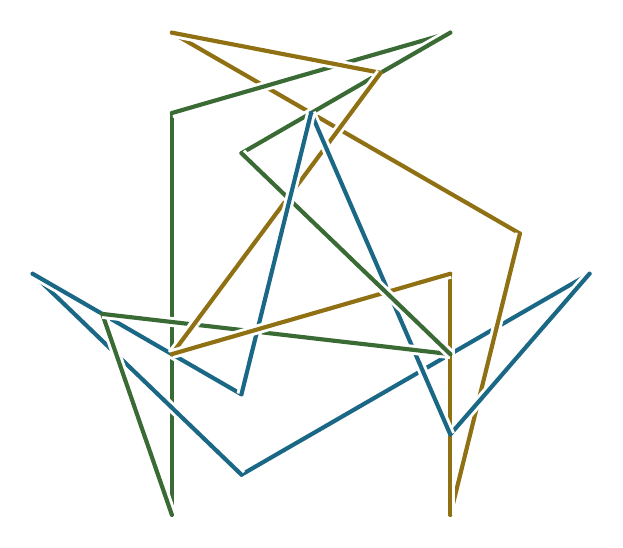
\begin{tikzpicture}
\draw[white,line width=3.6pt] (1.866,-2.665)--(1.768,-3.062);
\draw[ringC,line width=1.5pt,line cap=round] (1.866,-2.665)--(1.768,-3.062);
\draw[white,line width=3.6pt] (3.536,-0.000)--(3.044,-0.284);
\draw[ringB,line width=1.5pt,line cap=round] (3.536,-0.000)--(3.044,-0.284);
\draw[white,line width=3.6pt] (-3.241,-0.284)--(-3.536,0.000);
\draw[ringB,line width=1.5pt,line cap=round] (-3.241,-0.284)--(-3.536,0.000);
\draw[white,line width=3.6pt] (-1.768,3.062)--(-1.277,2.778);
\draw[ringC,line width=1.5pt,line cap=round] (-1.768,3.062)--(-1.277,2.778);
\draw[white,line width=3.6pt] (-1.768,-3.062)--(-1.768,-2.495);
\draw[ringD,line width=1.5pt,line cap=round] (-1.768,-3.062)--(-1.768,-2.495);
\draw[white,line width=3.6pt] (1.375,2.948)--(1.768,3.062);
\draw[ringD,line width=1.5pt,line cap=round] (1.375,2.948)--(1.768,3.062);
\draw[white,line width=3.6pt] (-1.473,3.005)--(-1.768,3.062);
\draw[ringC,line width=1.5pt,line cap=round] (-1.473,3.005)--(-1.768,3.062);
\draw[white,line width=3.6pt] (-1.866,-2.778)--(-1.768,-3.062);
\draw[ringD,line width=1.5pt,line cap=round] (-1.866,-2.778)--(-1.768,-3.062);
\draw[white,line width=3.6pt] (3.339,-0.227)--(3.536,-0.000);
\draw[ringB,line width=1.5pt,line cap=round] (3.339,-0.227)--(3.536,-0.000);
\draw[white,line width=3.6pt] (1.964,-2.268)--(1.866,-2.665);
\draw[ringC,line width=1.5pt,line cap=round] (1.964,-2.268)--(1.866,-2.665);
\draw[white,line width=3.6pt] (3.044,-0.284)--(2.553,-0.567);
\draw[ringB,line width=1.5pt,line cap=round] (3.044,-0.284)--(2.553,-0.567);
\draw[white,line width=3.6pt] (-2.946,-0.567)--(-3.241,-0.284);
\draw[ringB,line width=1.5pt,line cap=round] (-2.946,-0.567)--(-3.241,-0.284);
\draw[white,line width=3.6pt] (-3.536,0.000)--(-3.241,-0.170);
\draw[ringB,line width=1.5pt,line cap=round] (-3.536,0.000)--(-3.241,-0.170);
\draw[white,line width=3.6pt] (1.768,-3.062)--(1.768,-2.722);
\draw[ringC,line width=1.5pt,line cap=round] (1.768,-3.062)--(1.768,-2.722);
\draw[white,line width=3.6pt] (-1.277,2.778)--(-0.786,2.495);
\draw[ringC,line width=1.5pt,line cap=round] (-1.277,2.778)--(-0.786,2.495);
\draw[white,line width=3.6pt] (-1.768,-2.495)--(-1.768,-1.928);
\draw[ringD,line width=1.5pt,line cap=round] (-1.768,-2.495)--(-1.768,-1.928);
\draw[white,line width=3.6pt] (0.982,2.835)--(1.375,2.948);
\draw[ringD,line width=1.5pt,line cap=round] (0.982,2.835)--(1.375,2.948);
\draw[white,line width=3.6pt] (1.768,3.062)--(1.473,2.892);
\draw[ringD,line width=1.5pt,line cap=round] (1.768,3.062)--(1.473,2.892);
\draw[white,line width=3.6pt] (-2.652,-0.851)--(-2.946,-0.567);
\draw[ringB,line width=1.5pt,line cap=round] (-2.652,-0.851)--(-2.946,-0.567);
\draw[white,line width=3.6pt] (-0.786,2.495)--(-0.295,2.211);
\draw[ringC,line width=1.5pt,line cap=round] (-0.786,2.495)--(-0.295,2.211);
\draw[white,line width=3.6pt] (2.062,-1.871)--(1.964,-2.268);
\draw[ringC,line width=1.5pt,line cap=round] (2.062,-1.871)--(1.964,-2.268);
\draw[white,line width=3.6pt] (-1.768,-1.928)--(-1.768,-1.361);
\draw[ringD,line width=1.5pt,line cap=round] (-1.768,-1.928)--(-1.768,-1.361);
\draw[white,line width=3.6pt] (0.589,2.722)--(0.982,2.835);
\draw[ringD,line width=1.5pt,line cap=round] (0.589,2.722)--(0.982,2.835);
\draw[white,line width=3.6pt] (2.553,-0.567)--(2.062,-0.851);
\draw[ringB,line width=1.5pt,line cap=round] (2.553,-0.567)--(2.062,-0.851);
\draw[white,line width=3.6pt] (-1.179,2.948)--(-1.473,3.005);
\draw[ringC,line width=1.5pt,line cap=round] (-1.179,2.948)--(-1.473,3.005);
\draw[white,line width=3.6pt] (-1.964,-2.495)--(-1.866,-2.778);
\draw[ringD,line width=1.5pt,line cap=round] (-1.964,-2.495)--(-1.866,-2.778);
\draw[white,line width=3.6pt] (3.143,-0.454)--(3.339,-0.227);
\draw[ringB,line width=1.5pt,line cap=round] (3.143,-0.454)--(3.339,-0.227);
\draw[white,line width=3.6pt] (-2.357,-1.134)--(-2.652,-0.851);
\draw[ringB,line width=1.5pt,line cap=round] (-2.357,-1.134)--(-2.652,-0.851);
\draw[white,line width=3.6pt] (-0.295,2.211)--(0.196,1.928);
\draw[ringC,line width=1.5pt,line cap=round] (-0.295,2.211)--(0.196,1.928);
\draw[white,line width=3.6pt] (2.161,-1.474)--(2.062,-1.871);
\draw[ringC,line width=1.5pt,line cap=round] (2.161,-1.474)--(2.062,-1.871);
\draw[white,line width=3.6pt] (-1.768,-1.361)--(-1.768,-0.794);
\draw[ringD,line width=1.5pt,line cap=round] (-1.768,-1.361)--(-1.768,-0.794);
\draw[white,line width=3.6pt] (0.196,2.608)--(0.589,2.722);
\draw[ringD,line width=1.5pt,line cap=round] (0.196,2.608)--(0.589,2.722);
\draw[white,line width=3.6pt] (2.062,-0.851)--(1.571,-1.134);
\draw[ringB,line width=1.5pt,line cap=round] (2.062,-0.851)--(1.571,-1.134);
\draw[white,line width=3.6pt] (-2.062,-1.418)--(-2.357,-1.134);
\draw[ringB,line width=1.5pt,line cap=round] (-2.062,-1.418)--(-2.357,-1.134);
\draw[white,line width=3.6pt] (0.196,1.928)--(0.687,1.644);
\draw[ringC,line width=1.5pt,line cap=round] (0.196,1.928)--(0.687,1.644);
\draw[white,line width=3.6pt] (2.259,-1.077)--(2.161,-1.474);
\draw[ringC,line width=1.5pt,line cap=round] (2.259,-1.077)--(2.161,-1.474);
\draw[white,line width=3.6pt] (-1.768,-0.794)--(-1.768,-0.227);
\draw[ringD,line width=1.5pt,line cap=round] (-1.768,-0.794)--(-1.768,-0.227);
\draw[white,line width=3.6pt] (-0.196,2.495)--(0.196,2.608);
\draw[ringD,line width=1.5pt,line cap=round] (-0.196,2.495)--(0.196,2.608);
\draw[white,line width=3.6pt] (1.571,-1.134)--(1.080,-1.418);
\draw[ringB,line width=1.5pt,line cap=round] (1.571,-1.134)--(1.080,-1.418);
\draw[white,line width=3.6pt] (-3.241,-0.170)--(-2.946,-0.340);
\draw[ringB,line width=1.5pt,line cap=round] (-3.241,-0.170)--(-2.946,-0.340);
\draw[white,line width=3.6pt] (1.768,-2.722)--(1.768,-2.381);
\draw[ringC,line width=1.5pt,line cap=round] (1.768,-2.722)--(1.768,-2.381);
\draw[white,line width=3.6pt] (1.473,2.892)--(1.179,2.722);
\draw[ringD,line width=1.5pt,line cap=round] (1.473,2.892)--(1.179,2.722);
\draw[white,line width=3.6pt] (2.946,-0.680)--(3.143,-0.454);
\draw[ringB,line width=1.5pt,line cap=round] (2.946,-0.680)--(3.143,-0.454);
\draw[white,line width=3.6pt] (-0.884,2.892)--(-1.179,2.948);
\draw[ringC,line width=1.5pt,line cap=round] (-0.884,2.892)--(-1.179,2.948);
\draw[white,line width=3.6pt] (-2.062,-2.211)--(-1.964,-2.495);
\draw[ringD,line width=1.5pt,line cap=round] (-2.062,-2.211)--(-1.964,-2.495);
\draw[white,line width=3.6pt] (1.080,-1.418)--(0.589,-1.701);
\draw[ringB,line width=1.5pt,line cap=round] (1.080,-1.418)--(0.589,-1.701);
\draw[white,line width=3.6pt] (-1.768,-1.701)--(-2.062,-1.418);
\draw[ringB,line width=1.5pt,line cap=round] (-1.768,-1.701)--(-2.062,-1.418);
\draw[white,line width=3.6pt] (0.687,1.644)--(1.179,1.361);
\draw[ringC,line width=1.5pt,line cap=round] (0.687,1.644)--(1.179,1.361);
\draw[white,line width=3.6pt] (2.357,-0.680)--(2.259,-1.077);
\draw[ringC,line width=1.5pt,line cap=round] (2.357,-0.680)--(2.259,-1.077);
\draw[white,line width=3.6pt] (-1.768,-0.227)--(-1.768,0.340);
\draw[ringD,line width=1.5pt,line cap=round] (-1.768,-0.227)--(-1.768,0.340);
\draw[white,line width=3.6pt] (-0.589,2.381)--(-0.196,2.495);
\draw[ringD,line width=1.5pt,line cap=round] (-0.589,2.381)--(-0.196,2.495);
\draw[white,line width=3.6pt] (0.589,-1.701)--(0.098,-1.985);
\draw[ringB,line width=1.5pt,line cap=round] (0.589,-1.701)--(0.098,-1.985);
\draw[white,line width=3.6pt] (-1.473,-1.985)--(-1.768,-1.701);
\draw[ringB,line width=1.5pt,line cap=round] (-1.473,-1.985)--(-1.768,-1.701);
\draw[white,line width=3.6pt] (1.179,1.361)--(1.670,1.077);
\draw[ringC,line width=1.5pt,line cap=round] (1.179,1.361)--(1.670,1.077);
\draw[white,line width=3.6pt] (2.455,-0.284)--(2.357,-0.680);
\draw[ringC,line width=1.5pt,line cap=round] (2.455,-0.284)--(2.357,-0.680);
\draw[white,line width=3.6pt] (-1.768,0.340)--(-1.768,0.907);
\draw[ringD,line width=1.5pt,line cap=round] (-1.768,0.340)--(-1.768,0.907);
\draw[white,line width=3.6pt] (-0.982,2.268)--(-0.589,2.381);
\draw[ringD,line width=1.5pt,line cap=round] (-0.982,2.268)--(-0.589,2.381);
\draw[white,line width=3.6pt] (2.750,-0.907)--(2.946,-0.680);
\draw[ringB,line width=1.5pt,line cap=round] (2.750,-0.907)--(2.946,-0.680);
\draw[white,line width=3.6pt] (-0.589,2.835)--(-0.884,2.892);
\draw[ringC,line width=1.5pt,line cap=round] (-0.589,2.835)--(-0.884,2.892);
\draw[white,line width=3.6pt] (-2.161,-1.928)--(-2.062,-2.211);
\draw[ringD,line width=1.5pt,line cap=round] (-2.161,-1.928)--(-2.062,-2.211);
\draw[white,line width=3.6pt] (1.768,-2.381)--(1.768,-2.041);
\draw[ringC,line width=1.5pt,line cap=round] (1.768,-2.381)--(1.768,-2.041);
\draw[white,line width=3.6pt] (0.098,-1.985)--(-0.393,-2.268);
\draw[ringB,line width=1.5pt,line cap=round] (0.098,-1.985)--(-0.393,-2.268);
\draw[white,line width=3.6pt] (-2.946,-0.340)--(-2.652,-0.510);
\draw[ringB,line width=1.5pt,line cap=round] (-2.946,-0.340)--(-2.652,-0.510);
\draw[white,line width=3.6pt] (1.670,1.077)--(2.161,0.794);
\draw[ringC,line width=1.5pt,line cap=round] (1.670,1.077)--(2.161,0.794);
\draw[white,line width=3.6pt] (-1.768,0.907)--(-1.768,1.474);
\draw[ringD,line width=1.5pt,line cap=round] (-1.768,0.907)--(-1.768,1.474);
\draw[white,line width=3.6pt] (1.179,2.722)--(0.884,2.552);
\draw[ringD,line width=1.5pt,line cap=round] (1.179,2.722)--(0.884,2.552);
\draw[white,line width=3.6pt] (-1.179,-2.268)--(-1.473,-1.985);
\draw[ringB,line width=1.5pt,line cap=round] (-1.179,-2.268)--(-1.473,-1.985);
\draw[white,line width=3.6pt] (2.553,0.113)--(2.455,-0.284);
\draw[ringC,line width=1.5pt,line cap=round] (2.553,0.113)--(2.455,-0.284);
\draw[white,line width=3.6pt] (-1.375,2.155)--(-0.982,2.268);
\draw[ringD,line width=1.5pt,line cap=round] (-1.375,2.155)--(-0.982,2.268);
\draw[white,line width=3.6pt] (-0.393,-2.268)--(-0.884,-2.552);
\draw[ringB,line width=1.5pt,line cap=round] (-0.393,-2.268)--(-0.884,-2.552);
\draw[white,line width=3.6pt] (2.161,0.794)--(2.652,0.510);
\draw[ringC,line width=1.5pt,line cap=round] (2.161,0.794)--(2.652,0.510);
\draw[white,line width=3.6pt] (-1.768,1.474)--(-1.768,2.041);
\draw[ringD,line width=1.5pt,line cap=round] (-1.768,1.474)--(-1.768,2.041);
\draw[white,line width=3.6pt] (2.652,0.510)--(2.553,0.113);
\draw[ringC,line width=1.5pt,line cap=round] (2.652,0.510)--(2.553,0.113);
\draw[white,line width=3.6pt] (-0.884,-2.552)--(-1.179,-2.268);
\draw[ringB,line width=1.5pt,line cap=round] (-0.884,-2.552)--(-1.179,-2.268);
\draw[white,line width=3.6pt] (-1.768,2.041)--(-1.375,2.155);
\draw[ringD,line width=1.5pt,line cap=round] (-1.768,2.041)--(-1.375,2.155);
\draw[white,line width=3.6pt] (2.553,-1.134)--(2.750,-0.907);
\draw[ringB,line width=1.5pt,line cap=round] (2.553,-1.134)--(2.750,-0.907);
\draw[white,line width=3.6pt] (-0.295,2.778)--(-0.589,2.835);
\draw[ringC,line width=1.5pt,line cap=round] (-0.295,2.778)--(-0.589,2.835);
\draw[white,line width=3.6pt] (-2.259,-1.644)--(-2.161,-1.928);
\draw[ringD,line width=1.5pt,line cap=round] (-2.259,-1.644)--(-2.161,-1.928);
\draw[white,line width=3.6pt] (-2.652,-0.510)--(-2.357,-0.680);
\draw[ringB,line width=1.5pt,line cap=round] (-2.652,-0.510)--(-2.357,-0.680);
\draw[white,line width=3.6pt] (1.768,-2.041)--(1.768,-1.701);
\draw[ringC,line width=1.5pt,line cap=round] (1.768,-2.041)--(1.768,-1.701);
\draw[white,line width=3.6pt] (0.884,2.552)--(0.589,2.381);
\draw[ringD,line width=1.5pt,line cap=round] (0.884,2.552)--(0.589,2.381);
\draw[white,line width=3.6pt] (2.357,-1.361)--(2.553,-1.134);
\draw[ringB,line width=1.5pt,line cap=round] (2.357,-1.361)--(2.553,-1.134);
\draw[white,line width=3.6pt] (0.000,2.722)--(-0.295,2.778);
\draw[ringC,line width=1.5pt,line cap=round] (0.000,2.722)--(-0.295,2.778);
\draw[white,line width=3.6pt] (-2.357,-1.361)--(-2.259,-1.644);
\draw[ringD,line width=1.5pt,line cap=round] (-2.357,-1.361)--(-2.259,-1.644);
\draw[white,line width=3.6pt] (2.161,-1.588)--(2.357,-1.361);
\draw[ringB,line width=1.5pt,line cap=round] (2.161,-1.588)--(2.357,-1.361);
\draw[white,line width=3.6pt] (0.295,2.665)--(0.000,2.722);
\draw[ringC,line width=1.5pt,line cap=round] (0.295,2.665)--(0.000,2.722);
\draw[white,line width=3.6pt] (-2.455,-1.077)--(-2.357,-1.361);
\draw[ringD,line width=1.5pt,line cap=round] (-2.455,-1.077)--(-2.357,-1.361);
\draw[white,line width=3.6pt] (-2.357,-0.680)--(-2.062,-0.851);
\draw[ringB,line width=1.5pt,line cap=round] (-2.357,-0.680)--(-2.062,-0.851);
\draw[white,line width=3.6pt] (0.589,2.381)--(0.295,2.211);
\draw[ringD,line width=1.5pt,line cap=round] (0.589,2.381)--(0.295,2.211);
\draw[white,line width=3.6pt] (1.768,-1.701)--(1.768,-1.361);
\draw[ringC,line width=1.5pt,line cap=round] (1.768,-1.701)--(1.768,-1.361);
\draw[white,line width=3.6pt] (-2.553,-0.794)--(-2.455,-1.077);
\draw[ringD,line width=1.5pt,line cap=round] (-2.553,-0.794)--(-2.455,-1.077);
\draw[white,line width=3.6pt] (0.589,2.608)--(0.295,2.665);
\draw[ringC,line width=1.5pt,line cap=round] (0.589,2.608)--(0.295,2.665);
\draw[white,line width=3.6pt] (1.964,-1.814)--(2.161,-1.588);
\draw[ringB,line width=1.5pt,line cap=round] (1.964,-1.814)--(2.161,-1.588);
\draw[white,line width=3.6pt] (1.768,-1.361)--(1.768,-1.021);
\draw[ringC,line width=1.5pt,line cap=round] (1.768,-1.361)--(1.768,-1.021);
\draw[white,line width=3.6pt] (0.295,2.211)--(0.000,2.041);
\draw[ringD,line width=1.5pt,line cap=round] (0.295,2.211)--(0.000,2.041);
\draw[white,line width=3.6pt] (-2.062,-0.851)--(-1.768,-1.021);
\draw[ringB,line width=1.5pt,line cap=round] (-2.062,-0.851)--(-1.768,-1.021);
\draw[white,line width=3.6pt] (0.884,2.552)--(0.589,2.608);
\draw[ringC,line width=1.5pt,line cap=round] (0.884,2.552)--(0.589,2.608);
\draw[white,line width=3.6pt] (-2.652,-0.510)--(-2.553,-0.794);
\draw[ringD,line width=1.5pt,line cap=round] (-2.652,-0.510)--(-2.553,-0.794);
\draw[white,line width=3.6pt] (1.768,-2.041)--(1.964,-1.814);
\draw[ringB,line width=1.5pt,line cap=round] (1.768,-2.041)--(1.964,-1.814);
\draw[white,line width=3.6pt] (1.571,-1.588)--(1.768,-2.041);
\draw[ringB,line width=1.5pt,line cap=round] (1.571,-1.588)--(1.768,-2.041);
\draw[white,line width=3.6pt] (0.589,2.155)--(0.884,2.552);
\draw[ringC,line width=1.5pt,line cap=round] (0.589,2.155)--(0.884,2.552);
\draw[white,line width=3.6pt] (-2.161,-0.567)--(-2.652,-0.510);
\draw[ringD,line width=1.5pt,line cap=round] (-2.161,-0.567)--(-2.652,-0.510);
\draw[white,line width=3.6pt] (-1.768,-1.021)--(-1.473,-1.191);
\draw[ringB,line width=1.5pt,line cap=round] (-1.768,-1.021)--(-1.473,-1.191);
\draw[white,line width=3.6pt] (1.768,-1.021)--(1.768,-0.680);
\draw[ringC,line width=1.5pt,line cap=round] (1.768,-1.021)--(1.768,-0.680);
\draw[white,line width=3.6pt] (0.000,2.041)--(-0.295,1.871);
\draw[ringD,line width=1.5pt,line cap=round] (0.000,2.041)--(-0.295,1.871);
\draw[white,line width=3.6pt] (1.375,-1.134)--(1.571,-1.588);
\draw[ringB,line width=1.5pt,line cap=round] (1.375,-1.134)--(1.571,-1.588);
\draw[white,line width=3.6pt] (0.295,1.758)--(0.589,2.155);
\draw[ringC,line width=1.5pt,line cap=round] (0.295,1.758)--(0.589,2.155);
\draw[white,line width=3.6pt] (-1.670,-0.624)--(-2.161,-0.567);
\draw[ringD,line width=1.5pt,line cap=round] (-1.670,-0.624)--(-2.161,-0.567);
\draw[white,line width=3.6pt] (-1.473,-1.191)--(-1.179,-1.361);
\draw[ringB,line width=1.5pt,line cap=round] (-1.473,-1.191)--(-1.179,-1.361);
\draw[white,line width=3.6pt] (1.768,-0.680)--(1.768,-0.340);
\draw[ringC,line width=1.5pt,line cap=round] (1.768,-0.680)--(1.768,-0.340);
\draw[white,line width=3.6pt] (-0.295,1.871)--(-0.589,1.701);
\draw[ringD,line width=1.5pt,line cap=round] (-0.295,1.871)--(-0.589,1.701);
\draw[white,line width=3.6pt] (1.179,-0.680)--(1.375,-1.134);
\draw[ringB,line width=1.5pt,line cap=round] (1.179,-0.680)--(1.375,-1.134);
\draw[white,line width=3.6pt] (-0.000,1.361)--(0.295,1.758);
\draw[ringC,line width=1.5pt,line cap=round] (-0.000,1.361)--(0.295,1.758);
\draw[white,line width=3.6pt] (-1.179,-0.680)--(-1.670,-0.624);
\draw[ringD,line width=1.5pt,line cap=round] (-1.179,-0.680)--(-1.670,-0.624);
\draw[white,line width=3.6pt] (0.982,-0.227)--(1.179,-0.680);
\draw[ringB,line width=1.5pt,line cap=round] (0.982,-0.227)--(1.179,-0.680);
\draw[white,line width=3.6pt] (-0.295,0.964)--(-0.000,1.361);
\draw[ringC,line width=1.5pt,line cap=round] (-0.295,0.964)--(-0.000,1.361);
\draw[white,line width=3.6pt] (-0.687,-0.737)--(-1.179,-0.680);
\draw[ringD,line width=1.5pt,line cap=round] (-0.687,-0.737)--(-1.179,-0.680);
\draw[white,line width=3.6pt] (-1.179,-1.361)--(-0.884,-1.531);
\draw[ringB,line width=1.5pt,line cap=round] (-1.179,-1.361)--(-0.884,-1.531);
\draw[white,line width=3.6pt] (1.768,-0.340)--(1.768,0.000);
\draw[ringC,line width=1.5pt,line cap=round] (1.768,-0.340)--(1.768,0.000);
\draw[white,line width=3.6pt] (-0.589,1.701)--(-0.884,1.531);
\draw[ringD,line width=1.5pt,line cap=round] (-0.589,1.701)--(-0.884,1.531);
\draw[white,line width=3.6pt] (0.786,0.227)--(0.982,-0.227);
\draw[ringB,line width=1.5pt,line cap=round] (0.786,0.227)--(0.982,-0.227);
\draw[white,line width=3.6pt] (-0.589,0.567)--(-0.295,0.964);
\draw[ringC,line width=1.5pt,line cap=round] (-0.589,0.567)--(-0.295,0.964);
\draw[white,line width=3.6pt] (-0.196,-0.794)--(-0.687,-0.737);
\draw[ringD,line width=1.5pt,line cap=round] (-0.196,-0.794)--(-0.687,-0.737);
\draw[white,line width=3.6pt] (1.768,0.000)--(1.375,-0.113);
\draw[ringC,line width=1.5pt,line cap=round] (1.768,0.000)--(1.375,-0.113);
\draw[white,line width=3.6pt] (-0.884,1.531)--(-0.589,1.247);
\draw[ringD,line width=1.5pt,line cap=round] (-0.884,1.531)--(-0.589,1.247);
\draw[white,line width=3.6pt] (-0.884,-1.531)--(-0.786,-1.134);
\draw[ringB,line width=1.5pt,line cap=round] (-0.884,-1.531)--(-0.786,-1.134);
\draw[white,line width=3.6pt] (-0.786,-1.134)--(-0.687,-0.737);
\draw[ringB,line width=1.5pt,line cap=round] (-0.786,-1.134)--(-0.687,-0.737);
\draw[white,line width=3.6pt] (1.375,-0.113)--(0.982,-0.227);
\draw[ringC,line width=1.5pt,line cap=round] (1.375,-0.113)--(0.982,-0.227);
\draw[white,line width=3.6pt] (-0.589,1.247)--(-0.295,0.964);
\draw[ringD,line width=1.5pt,line cap=round] (-0.589,1.247)--(-0.295,0.964);
\draw[white,line width=3.6pt] (0.589,0.680)--(0.786,0.227);
\draw[ringB,line width=1.5pt,line cap=round] (0.589,0.680)--(0.786,0.227);
\draw[white,line width=3.6pt] (-0.884,0.170)--(-0.589,0.567);
\draw[ringC,line width=1.5pt,line cap=round] (-0.884,0.170)--(-0.589,0.567);
\draw[white,line width=3.6pt] (0.295,-0.851)--(-0.196,-0.794);
\draw[ringD,line width=1.5pt,line cap=round] (0.295,-0.851)--(-0.196,-0.794);
\draw[white,line width=3.6pt] (-0.687,-0.737)--(-0.589,-0.340);
\draw[ringB,line width=1.5pt,line cap=round] (-0.687,-0.737)--(-0.589,-0.340);
\draw[white,line width=3.6pt] (0.982,-0.227)--(0.589,-0.340);
\draw[ringC,line width=1.5pt,line cap=round] (0.982,-0.227)--(0.589,-0.340);
\draw[white,line width=3.6pt] (-0.295,0.964)--(0.000,0.680);
\draw[ringD,line width=1.5pt,line cap=round] (-0.295,0.964)--(0.000,0.680);
\draw[white,line width=3.6pt] (-0.589,-0.340)--(-0.491,0.057);
\draw[ringB,line width=1.5pt,line cap=round] (-0.589,-0.340)--(-0.491,0.057);
\draw[white,line width=3.6pt] (0.589,-0.340)--(0.196,-0.454);
\draw[ringC,line width=1.5pt,line cap=round] (0.589,-0.340)--(0.196,-0.454);
\draw[white,line width=3.6pt] (0.000,0.680)--(0.295,0.397);
\draw[ringD,line width=1.5pt,line cap=round] (0.000,0.680)--(0.295,0.397);
\draw[white,line width=3.6pt] (0.393,1.134)--(0.589,0.680);
\draw[ringB,line width=1.5pt,line cap=round] (0.393,1.134)--(0.589,0.680);
\draw[white,line width=3.6pt] (-1.179,-0.227)--(-0.884,0.170);
\draw[ringC,line width=1.5pt,line cap=round] (-1.179,-0.227)--(-0.884,0.170);
\draw[white,line width=3.6pt] (0.786,-0.907)--(0.295,-0.851);
\draw[ringD,line width=1.5pt,line cap=round] (0.786,-0.907)--(0.295,-0.851);
\draw[white,line width=3.6pt] (-0.491,0.057)--(-0.393,0.454);
\draw[ringB,line width=1.5pt,line cap=round] (-0.491,0.057)--(-0.393,0.454);
\draw[white,line width=3.6pt] (0.196,-0.454)--(-0.196,-0.567);
\draw[ringC,line width=1.5pt,line cap=round] (0.196,-0.454)--(-0.196,-0.567);
\draw[white,line width=3.6pt] (0.295,0.397)--(0.589,0.113);
\draw[ringD,line width=1.5pt,line cap=round] (0.295,0.397)--(0.589,0.113);
\draw[white,line width=3.6pt] (-0.393,0.454)--(-0.295,0.851);
\draw[ringB,line width=1.5pt,line cap=round] (-0.393,0.454)--(-0.295,0.851);
\draw[white,line width=3.6pt] (-0.196,-0.567)--(-0.589,-0.680);
\draw[ringC,line width=1.5pt,line cap=round] (-0.196,-0.567)--(-0.589,-0.680);
\draw[white,line width=3.6pt] (0.589,0.113)--(0.884,-0.170);
\draw[ringD,line width=1.5pt,line cap=round] (0.589,0.113)--(0.884,-0.170);
\draw[white,line width=3.6pt] (-1.473,-0.624)--(-1.179,-0.227);
\draw[ringC,line width=1.5pt,line cap=round] (-1.473,-0.624)--(-1.179,-0.227);
\draw[white,line width=3.6pt] (1.277,-0.964)--(0.786,-0.907);
\draw[ringD,line width=1.5pt,line cap=round] (1.277,-0.964)--(0.786,-0.907);
\draw[white,line width=3.6pt] (0.196,1.588)--(0.393,1.134);
\draw[ringB,line width=1.5pt,line cap=round] (0.196,1.588)--(0.393,1.134);
\draw[white,line width=3.6pt] (-0.295,0.851)--(-0.196,1.247);
\draw[ringB,line width=1.5pt,line cap=round] (-0.295,0.851)--(-0.196,1.247);
\draw[white,line width=3.6pt] (-0.589,-0.680)--(-0.982,-0.794);
\draw[ringC,line width=1.5pt,line cap=round] (-0.589,-0.680)--(-0.982,-0.794);
\draw[white,line width=3.6pt] (0.884,-0.170)--(1.179,-0.454);
\draw[ringD,line width=1.5pt,line cap=round] (0.884,-0.170)--(1.179,-0.454);
\draw[white,line width=3.6pt] (-0.196,1.247)--(-0.098,1.644);
\draw[ringB,line width=1.5pt,line cap=round] (-0.196,1.247)--(-0.098,1.644);
\draw[white,line width=3.6pt] (-0.982,-0.794)--(-1.375,-0.907);
\draw[ringC,line width=1.5pt,line cap=round] (-0.982,-0.794)--(-1.375,-0.907);
\draw[white,line width=3.6pt] (1.179,-0.454)--(1.473,-0.737);
\draw[ringD,line width=1.5pt,line cap=round] (1.179,-0.454)--(1.473,-0.737);
\draw[white,line width=3.6pt] (0.000,2.041)--(0.196,1.588);
\draw[ringB,line width=1.5pt,line cap=round] (0.000,2.041)--(0.196,1.588);
\draw[white,line width=3.6pt] (-1.768,-1.021)--(-1.473,-0.624);
\draw[ringC,line width=1.5pt,line cap=round] (-1.768,-1.021)--(-1.473,-0.624);
\draw[white,line width=3.6pt] (1.768,-1.021)--(1.277,-0.964);
\draw[ringD,line width=1.5pt,line cap=round] (1.768,-1.021)--(1.277,-0.964);
\draw[white,line width=3.6pt] (-0.098,1.644)--(0.000,2.041);
\draw[ringB,line width=1.5pt,line cap=round] (-0.098,1.644)--(0.000,2.041);
\draw[white,line width=3.6pt] (-1.375,-0.907)--(-1.768,-1.021);
\draw[ringC,line width=1.5pt,line cap=round] (-1.375,-0.907)--(-1.768,-1.021);
\draw[white,line width=3.6pt] (1.473,-0.737)--(1.768,-1.021);
\draw[ringD,line width=1.5pt,line cap=round] (1.473,-0.737)--(1.768,-1.021);
\end{tikzpicture}
}
\caption{The sublink obtained by deleting \textcolor{ringA}{$K_1$}. By
Lemma~\ref{lem:vertices} the three surviving
components are those belonging to the faces meeting at $v_1$, and by
Proposition~\ref{prop:sublinks} they form the Borromean rings. The other three
sublinks are carried onto this one by the symmetry.}
\label{fig:sublink}
\end{figure}

\section{Remarks}\label{sec:remarks}

\paragraph{What is and is not proved.}
The symmetry in Theorem~\ref{thm:main} is exact and is established by
Lemma~\ref{lem:generate} rather than measured; the vanishing of the pairwise
linking numbers is a finite exact computation. The identification of the
sublinks as $\Bor$, however, rests on Proposition~\ref{prop:sublinks}, which
appeals to the tabulation of links of small crossing number. A synthetic
argument --- an explicit isotopy carrying one sublink onto the standard diagram
of $\Bor$, which by Lemma~\ref{lem:vertices} would settle all four at once ---
would be preferable, and we do not have one. The natural route is to redesign the component so that the Borromean
weave is visible in a neighbourhood of each vertex and the connecting arcs
demonstrably meet nothing.

\paragraph{Economy.}
Theorem~\ref{thm:minimal} rules out $12$ crossings. The link of
Theorem~\ref{thm:main} is far from that bound: its best projection among $192$
sampled directions has $36$ crossings. We make no claim about the minimal
crossing number of this link, nor about whether the link of
Theorem~\ref{thm:main} is the simplest one satisfying
Problem~\ref{prob:main}.

\bigskip
\noindent\textbf{Acknowledgement.} The observation that the four components
should be indexed by the faces of a tetrahedron, so that triples of components
correspond to vertices, is due to Kyle Miller~\cite{miller2018}.

\bibliographystyle{plain}
\bibliography{refs}

\end{document}
